% !TeX spellcheck = pl_PL
%%%%%%%%%%%%%%%%%%%%%%%%%%%%%%%%%%%%%%%%%%%
%                                        %
% Szablon pracy dyplomowej inzynierskiej %
% zgodny  z aktualnymi  przepisami  SZJK %
%                                        %
%%%%%%%%%%%%%%%%%%%%%%%%%%%%%%%%%%%%%%%%%%
%                                        %
%  (c) Krzysztof Simiński, 2018-2023     %
%                                        %
%%%%%%%%%%%%%%%%%%%%%%%%%%%%%%%%%%%%%%%%%%
%                                        %
% Najnowsza wersja szablonów jest        %
% podstępna pod adresem                  %
% github.com/ksiminski/polsl-aei-theses  %
%                                        %
%%%%%%%%%%%%%%%%%%%%%%%%%%%%%%%%%%%%%%%%%%
%
%
% Projekt LaTeXowy zapewnia odpowiednie formatowanie pracy,
% zgodnie z wymaganiami Systemu zapewniania jakości kształcenia.
% Proszę nie zmieniać ustawień formatowania (np. fontu,
% marginesów, wytłuszczeń, kursywy itd. ).
%
% Projekt można kompilować na kilka sposobów.
%
% 1. kompilacja pdfLaTeX
%
% pdflatex main
% bibtex   main
% pdflatex main
% pdflatex main
%
%
% 2. kompilacja XeLaTeX
%
% Kompilatacja przy użyciu XeLaTeXa różni się tym, że na stronie
% tytułowej używany jest font Calibri. Wymaga to jego uprzedniego
% zainstalowania.
%
% xelatex main
% bibtex  main
% xelatex main
% xelatex main
%
%
%%%%%%%%%%%%%%%%%%%%%%%%%%%%%%%%%%%%%%%%%%%%%%%%%%%%%
% W przypadku pytań, uwag, proszę pisać na adres:   %
%      krzysztof.siminski(małpa)polsl.pl            %
%%%%%%%%%%%%%%%%%%%%%%%%%%%%%%%%%%%%%%%%%%%%%%%%%%%%%
%
% Chcemy ulepszać szablony LaTeXowe prac dyplomowych.
% Wypełniając ankietę spod poniższego adresu pomogą
% Państwo nam to zrobić. Ankieta jest całkowicie
% anonimowa. Dziękujemy!


% https://docs.google.com/forms/d/e/1FAIpQLScyllVxNKzKFHfILDfdbwC-jvT8YL0RSTFs-s27UGw9CKn-fQ/viewform?usp=sf_link
%
%%%%%%%%%%%%%%%%%%%%%%%%%%%%%%%%%%%%%%%%%%%%%%%%%%%%%%%%%%%%%%%%%%%%%%%%%

%%%%%%%%%%%%%%%%%%%%%%%%%%%%%%%%%%%%%%%%%%%%%%%
%                                             %
% PERSONALIZACJA PRACY – DANE PRACY           %
%                                             %
%%%%%%%%%%%%%%%%%%%%%%%%%%%%%%%%%%%%%%%%%%%%%%%

% Proszę wpisać swoje dane w poniższych definicjach.

% dane autora
\newcommand{\FirstNameAuthor}{Jacek}
\newcommand{\SurnameAuthor}{Cytera}
\newcommand{\IdAuthor}{295622}   % numer albumu  (bez $\langle$ i $\rangle$)

% drugi autor:
%\newcommand{\FirstNameCoauthor}{Imię}   % Jeżeli jest drugi autor, to tutaj należy podać imię.
%\newcommand{\SurnameCoauthor}{Nazwisko} % Jeżeli jest drugi autor, to tutaj należy podać nazwisko.
%\newcommand{\IdCoauthor}{$\langle$wpisać właściwy$\rangle$}  % numer albumu drugiego autora (bez $\langle$ i $\rangle$)
% Gdy nie ma drugiego autora, należy zostawić poniższe definicje puste, jak poniżej. Gdy jest drugi autor, należy zakomentować te linie.
\newcommand{\FirstNameCoauthor}{} % Jeżeli praca ma tylko jednego autora, to dane drugiego autora zostają puste.
\newcommand{\SurnameCoauthor}{}   % Jeżeli praca ma tylko jednego autora, to dane drugiego autora zostają puste.
\newcommand{\IdCoauthor}{}  % Jeżeli praca ma tylko jednego autora, to dane drugiego autora zostają puste.
%%%%%%%%%%

\newcommand{\Supervisor}{Dr hab. inż. prof. PŚ Adam Domański}     % dane promotora (bez $\langle$ i $\rangle$)
\newcommand{\Title}{Serwis do zarządzania notatkami w języku RUST}           % tytuł pracy po polsku
\newcommand{\TitleAlt}{Note management service in RUST}                     % thesis title in English
\newcommand{\Program}{Informatyka}            % kierunek studiów  (bez $\langle$ i $\rangle$)
\newcommand{\Specialisation}{Bazy Danych i Inżynieria Systemów}     % specjalność  (bez $\langle$ i $\rangle$)
\newcommand{\Departament}{Katedra Systemów Rozproszonych i Urządzeń Informatyki}        % katedra promotora  (bez $\langle$ i $\rangle$)

% Jeżeli został wyznaczony promotor pomocniczy lub opiekun, proszę go/ją wpisać ...
% \newcommand{\Consultant}{$\langle$stopień naukowy imię i nazwisko$\rangle$} % dane promotora pomocniczego, opiekuna (bez $\langle$ i $\rangle$)
% ... w przeciwnym razie proszę zostawić puste miejsce jak poniżej:
\newcommand{\Consultant}{} % brak promotowa pomocniczego / opiekuna

% koniec fragmentu do modyfikacji
%%%%%%%%%%%%%%%%%%%%%%%%%%%%%%%%%%%%%%%%%%


%%%%%%%%%%%%%%%%%%%%%%%%%%%%%%%%%%%%%%%%%%%%%%%
%                                             %
% KONIEC PERSONALIZACJI PRACY                 %
%                                             %
%%%%%%%%%%%%%%%%%%%%%%%%%%%%%%%%%%%%%%%%%%%%%%%

%%%%%%%%%%%%%%%%%%%%%%%%%%%%%%%%%%%%%%%%


%%%%%%%%%%%%%%%%%%%%%%%%%%%%%%%%%%%%%%%%%%%%%%%
%                                             %
% PROSZĘ NIE MODYFIKOWAĆ PONIŻSZYCH USTAWIEŃ! %
%                                             %
%%%%%%%%%%%%%%%%%%%%%%%%%%%%%%%%%%%%%%%%%%%%%%%



\documentclass[a4paper,twoside,12pt]{book}
\usepackage[utf8]{inputenc}                                      
\usepackage[T1]{fontenc}  
\usepackage{amsmath,amsfonts,amssymb,amsthm}
\usepackage[british,polish]{babel} 
\usepackage{indentfirst}
\usepackage{xurl}
\usepackage{xstring}
\usepackage{ifthen}
\usepackage{float}



\usepackage{ifxetex}

\ifxetex
	\usepackage{fontspec}
	\defaultfontfeatures{Mapping=tex—text} % to support TeX conventions like ``——-''
	\usepackage{xunicode} % Unicode support for LaTeX character names (accents, European chars, etc)
	\usepackage{xltxtra} % Extra customizations for XeLaTeX
\else
	\usepackage{lmodern}
\fi



\usepackage[margin=2.5cm]{geometry}
\usepackage{graphicx} 
\usepackage{hyperref}
\usepackage{booktabs}
\usepackage{tikz}
\usepackage{pgfplots}
\usepackage{mathtools}
\usepackage{geometry}
\usepackage{subcaption}   % subfigures
\usepackage[page]{appendix} % toc,
\renewcommand{\appendixtocname}{Dodatki}
\renewcommand{\appendixpagename}{Dodatki}
\renewcommand{\appendixname}{Dodatek}

\usepackage{csquotes}
\usepackage[natbib=true,backend=bibtex,maxbibnames=99]{biblatex}  % kompilacja bibliografii BibTeXem
%\usepackage[natbib=true,backend=biber,maxbibnames=99]{biblatex}  % kompilacja bibliografii Biberem
\bibliography{biblio}

\usepackage{ifmtarg}   % empty commands  

\usepackage{setspace}
\onehalfspacing


\frenchspacing



%%%% TODO LIST GENERATOR %%%%%%%%%

\usepackage{color}
\definecolor{brickred}      {cmyk}{0   , 0.89, 0.94, 0.28}

\makeatletter \newcommand \kslistofremarks{\section*{Uwagi} \@starttoc{rks}}
  \newcommand\l@uwagas[2]
    {\par\noindent \textbf{#2:} %\parbox{10cm}
{#1}\par} \makeatother


\newcommand{\ksremark}[1]{%
{%\marginpar{\textdbend}
{\color{brickred}{[#1]}}}%
\addcontentsline{rks}{uwagas}{\protect{#1}}%
}

\newcommand{\comma}{\ksremark{przecinek}}
\newcommand{\nocomma}{\ksremark{bez przecinka}}
\newcommand{\styl}{\ksremark{styl}}
\newcommand{\ortografia}{\ksremark{ortografia}}
\newcommand{\fleksja}{\ksremark{fleksja}}
\newcommand{\pauza}{\ksremark{pauza `--', nie dywiz `-'}}
\newcommand{\kolokwializm}{\ksremark{kolokwializm}}
\newcommand{\cudzyslowy}{\ksremark{,,polskie cudzysłowy''}}

%%%%%%%%%%%%%% END OF TODO LIST GENERATOR %%%%%%%%%%%

\newcommand{\printCoauthor}{%		
    \StrLen{\FirstNameCoauthor}[\FNCoALen]
    \ifthenelse{\FNCoALen > 0}%
    {%
		{\large\bfseries\Coauthor\par}
	
		{\normalsize\bfseries \LeftId: \IdCoauthor\par}
    }%
    {}
} 

%%%%%%%%%%%%%%%%%%%%%
\newcommand{\autor}{%		
    \StrLen{\FirstNameCoauthor}[\FNCoALenXX]
    \ifthenelse{\FNCoALenXX > 0}%
    {\FirstNameAuthor\ \SurnameAuthor, \FirstNameCoauthor\ \SurnameCoauthor}%
	{\FirstNameAuthor\ \SurnameAuthor}%
}
%%%%%%%%%%%%%%%%%%%%%

\StrLen{\FirstNameCoauthor}[\FNCoALen]
\ifthenelse{\FNCoALen > 0}%
{%
\author{\FirstNameAuthor\ \SurnameAuthor, \FirstNameCoauthor\ \SurnameCoauthor}
}%
{%
\author{\FirstNameAuthor\ \SurnameAuthor}
}%

%%%%%%%%%%%% ZYWA PAGINA %%%%%%%%%%%%%%%
% brak kapitalizacji zywej paginy
\usepackage{fancyhdr}
\pagestyle{fancy}
\fancyhf{}
\fancyhead[LO]{\nouppercase{\it\rightmark}}
\fancyhead[RE]{\nouppercase{\it\leftmark}}
\fancyhead[LE,RO]{\it\thepage}


\fancypagestyle{tylkoNumeryStron}{%
   \fancyhf{} 
   \fancyhead[LE,RO]{\it\thepage}
}

\fancypagestyle{bezNumeracji}{%
   \fancyhf{} 
   \fancyhead[LE,RO]{}
}


\fancypagestyle{NumeryStronNazwyRozdzialow}{%
   \fancyhf{} 
   \fancyhead[LE]{\nouppercase{\autor}}
   \fancyhead[RO]{\nouppercase{\leftmark}} 
   \fancyfoot[CE, CO]{\thepage}
}


%%%%%%%%%%%%% OBCE WTRETY  
\newcommand{\obcy}[1]{\emph{#1}}
\newcommand{\english}[1]{{\selectlanguage{british}\obcy{#1}}}
%%%%%%%%%%%%%%%%%%%%%%%%%%%%%

% polskie oznaczenia funkcji matematycznych
\renewcommand{\tan}{\operatorname {tg}}
\renewcommand{\log}{\operatorname {lg}}

% jeszcze jakies drobiazgi

\newcounter{stronyPozaNumeracja}

%%%%%%%%%%%%%%%%%%%%%%%%%%% 
\newcommand{\printOpiekun}[1]{%		

    \StrLen{\Consultant}[\mystringlen]
    \ifthenelse{\mystringlen > 0}%
    {%
       {\large{\bfseries OPIEKUN, PROMOTOR POMOCNICZY}\par}
       
       {\large{\bfseries \Consultant}\par}
    }%
    {}
} 
%
%%%%%%%%%%%%%%%%%%%%%%%%%%%%%%%%%%%%%%%%%%%%%%
 
% Proszę nie modyfikować poniższych definicji!
\newcommand{\Author}{\FirstNameAuthor\ \MakeUppercase{\SurnameAuthor}} 
\newcommand{\Coauthor}{\FirstNameCoauthor\ \MakeUppercase{\SurnameCoauthor}}
\newcommand{\Type}{PROJEKT INŻYNIERSKI}
\newcommand{\Faculty}{Wydział Automatyki, Elektroniki i Informatyki} 
\newcommand{\Polsl}{Politechnika Śląska}
\newcommand{\Logo}{politechnika_sl_logo_bw_pion_pl.pdf}
\newcommand{\LeftId}{Nr albumu}
\newcommand{\LeftProgram}{Kierunek}
\newcommand{\LeftSpecialisation}{Specjalność}
\newcommand{\LeftSUPERVISOR}{PROWADZĄCY PRACĘ}
\newcommand{\LeftDEPARTMENT}{KATEDRA}
%%%%%%%%%%%%%%%%%%%%%%%%%%%%%%%%%%%%%%%%%%%%%%

%%%%%%%%%%%%%%%%%%%%%%%%%%%%%%%%%%%%%%%%%%%%%%%
%                                             %
% KONIEC USTAWIEŃ                             %
%                                             %
%%%%%%%%%%%%%%%%%%%%%%%%%%%%%%%%%%%%%%%%%%%%%%%




%%%%%%%%%%%%%%%%%%%%%%%%%%%%%%%%%%%%%%%%%%%%%%%
%                                             %
% MOJE PAKIETY, USTAWIENIA ITD                %
%                                             %
%%%%%%%%%%%%%%%%%%%%%%%%%%%%%%%%%%%%%%%%%%%%%%%

% Tutaj proszę umieszczać swoje pakiety, makra, ustawienia itd.


 
%%%%%%%%%%%%%%%%%%%%%%%%%%%%%%%%%%%%%%%%%%%%%%%%%%%%%%%%%%%%%%%%%%%%%
% listingi i fragmentu kodu źródłowego 
% pakiet: listings lub minted
% % % % % % % % % % % % % % % % % % % % % % % % % % % % % % % % % % % 

% biblioteka listings
\usepackage{listings}
\lstset{%
morekeywords={string,exception,std,vector},% słowa kluczowe rozpoznawane przez pakiet listings
language=C++,% C, Matlab, Python, SQL, TeX, XML, bash, ... – vide https://www.ctan.org/pkg/listings
commentstyle=\textit,%
identifierstyle=\textsf,%
keywordstyle=\sffamily\bfseries, %\texttt, %
%captionpos=b,%
tabsize=3,%
frame=lines,%
numbers=left,%
numberstyle=\tiny,%
numbersep=5pt,%
breaklines=true,%
escapeinside={@*}{*@},%
}

% % % % % % % % % % % % % % % % % % % % % % % % % % % % % % % % % % % 
% pakiet minted
%\usepackage{minted}

% pakiet wymaga specjalnego kompilowania:
% pdflatex -shell-escape main.tex
% xelatex  -shell-escape main.tex

%\usepackage[chapter]{minted} % [section]
%%\usemintedstyle{bw}   % czarno-białe kody 
%
%\setminted % https://ctan.org/pkg/minted
%{
%%fontsize=\normalsize,%\footnotesize,
%%captionpos=b,%
%tabsize=3,%
%frame=lines,%
%framesep=2mm,
%numbers=left,%
%numbersep=5pt,%
%breaklines=true,%
%escapeinside=@@,%
%}

%%%%%%%%%%%%%%%%%%%%%%%%%%%%%%%%%%%%%%%%%%%%%%%%%%%%%%%%%%%%%%%%%%%%%



%%%%%%%%%%%%%%%%%%%%%%%%%%%%%%%%%%%%%%%%%%%%%%%
%                                             %
% KONIEC MOICH USTAWIEŃ                       %
%                                             %
%%%%%%%%%%%%%%%%%%%%%%%%%%%%%%%%%%%%%%%%%%%%%%%



%%%%%%%%%%%%%%%%%%%%%%%%%%%%%%%%%%%%%%%%


\begin{document}
%\kslistofremarks

\frontmatter

%%%%%%%%%%%%%%%%%%%%%%%%%%%%%%%%%%%%%%%%%%%%%%%
%                                             %
% PROSZĘ NIE MODYFIKOWAĆ STRONY TYTUŁOWEJ!    %
%                                             %
%%%%%%%%%%%%%%%%%%%%%%%%%%%%%%%%%%%%%%%%%%%%%%%


%%%%%%%%%%%%%%%%%%  STRONA TYTUŁOWA %%%%%%%%%%%%%%%%%%%
\pagestyle{empty}
{
	\newgeometry{top=1.5cm,%
	             bottom=2.5cm,%
	             left=3cm,
	             right=2.5cm}
 
	\ifxetex 
	  \begingroup
	  \setsansfont{Calibri}
	   
	\fi 
	 \sffamily
	\begin{center}
	\includegraphics[width=50mm]{\Logo}
	 
	
	{\Large\bfseries\Type\par}
	
	\vfill  \vfill  
			 
	{\large\Title\par}
	
	\vfill  
		
	{\large\bfseries\Author\par}
	
	{\normalsize\bfseries \LeftId: \IdAuthor}

	\printCoauthor
	
	\vfill  		
 
	{\large{\bfseries \LeftProgram:} \Program\par} 
	
	{\large{\bfseries \LeftSpecialisation:} \Specialisation\par} 
	 		
	\vfill  \vfill 	\vfill 	\vfill 	\vfill 	\vfill 	\vfill  
	 
	{\large{\bfseries \LeftSUPERVISOR}\par}
	
	{\large{\bfseries \Supervisor}\par}
				
	{\large{\bfseries \LeftDEPARTMENT\ \Departament} \par}
		
	{\large{\bfseries \Faculty}\par}
		
	\vfill  \vfill  

    	
    \printOpiekun{\Consultant}
    
	\vfill  \vfill  
		
    {\large\bfseries  Gliwice \the\year}

   \end{center}	
       \ifxetex 
       	  \endgroup
       \fi
	\restoregeometry
}
  
%%%%%%%%%%%%%%%%%%%%%%%%%%%%%%%%%%%%%%%%%%%%%%%
%                                             %
% KONIEC STRONY TYTUŁOWEJ                     %
%                                             %
%%%%%%%%%%%%%%%%%%%%%%%%%%%%%%%%%%%%%%%%%%%%%%%  


\cleardoublepage

\rmfamily\normalfont
\pagestyle{empty}


%%% No to zaczynamy pisać pracę :-) %%%%

\subsubsection*{Serwis do zarządzania notatkami w języku RUST} 
\Title

\subsubsection*{Streszczenie}  
Aplikacja  ma  na  celu  demostrację  możliwości  języka  Rust  do  programowania  aplikacji
internetowej, od strony zarówno serwera jak i klienta. W tym celu zostanie stworzony serwis do zarządzania
notatkami, z następującą funkcjonalnością:   

- tworzenie nowej notatki

- modyfikacja istniejącej notatki

- wyświetlenie wszystkich notatek

- usuwanie notatki

- tworzenie konta i logowanie użytkownika

- wyświetlanie profilu użytkownika

- zmiana danych użytkownika

- usuwanie konta użytkownika


\subsubsection*{Słowa kluczowe} 
aplikacja,rust,yew,axum,klient,serwer

\subsubsection*{Note management service in RUST} 
\begin{otherlanguage}{british}
\TitleAlt
\end{otherlanguage}

\subsubsection*{Abstract} 
\begin{otherlanguage}{british}
Application is meant to demonstrate the capabilities of Rust language for server
and client side web application development. In order to achieve this a note
management service will be created, with following features:

- creating new note

- updating existing note

- displaying all notes

- deleting existing note

- user creation and login

- displaying user profile

- updating user data

- deleting user account


\end{otherlanguage}
\subsubsection*{Key words}  
\begin{otherlanguage}{british}
webapplication,rust,yew,axum,frontend,backend
\end{otherlanguage}




%%%%%%%%%%%%%%%%%% SPIS TRESCI %%%%%%%%%%%%%%%%%%%%%%
% Add \thispagestyle{empty} to the toc file (main.toc), because \pagestyle{empty} doesn't work if the TOC has multiple pages
\addtocontents{toc}{\protect\thispagestyle{empty}}
\tableofcontents

%%%%%%%%%%%%%%%%%%%%%%%%%%%%%%%%%%%%%%%%%%%%%%%%%%%%%
\setcounter{stronyPozaNumeracja}{\value{page}}
\mainmatter
\pagestyle{empty}

\cleardoublepage

\pagestyle{NumeryStronNazwyRozdzialow}

%%%%%%%%%%%%%% wlasciwa tresc pracy %%%%%%%%%%%%%%%%%

\chapter{Wstęp}
\label{ch:wstep}

Serwis do zarządzania notatkami w języku Rust stanowi odpowiedź na rosnące potrzeby efektywnego zarządzania informacjami w dzisiejszym środowisku pracy. Wprowadzenie tego rodzaju narzędzia wiąże się z koniecznością ułatwienia organizacji i wyszukiwania notatek w sposób spójny i intuicyjny. Analiza aktualnych narzędzi tego typu pozwala zidentyfikować luki i potrzeby, które można skutecznie adresować za pomocą nowoczesnych technologii, takich jak Rust, aby stworzyć bardziej wydajne i bezpieczne rozwiązanie.

\hfill\break
Problem zarządzania notatkami jest szczególnie istotny w kontekście współczesnego środowiska pracy, gdzie ilość informacji, z jaką się stykamy, stale rośnie. Wykorzystanie języka Rust pozwala na tworzenie rozwiązań, które spełniają potrzeby bezpieczeństwa i szybkości działania (responsywności) tworzonych aplikacji. 

\hfill\break
Celem pracy inżynierskiej jest zaprojektowanie, implementacja i ocena serwisu do zarządzania notatkami opartego na języku Rust oraz technologiach axum.rs i yew.rs. Koncentrując się na aspektach praktycznych i technologicznych, praca ma na celu dostarczenie nowoczesnego narzędzia, które spełni oczekiwania użytkowników w zakresie prostoty obsługi, szybkości działania i bezpieczeństwa danych.

\hfill\break
Praca obejmuje zaprojektowanie serwisu, który umożliwi tworzenie, modyfikowanie i usuwanie notatek, a także przejrzyste ich wyśwetlanie. Ponad to aplikacja ma rozróżniać między użytkownikami i ich notatkami, oraz chronić dostęp do informacji przekazanych przez użytkowników aplikacji (czy to w formie notatek, czy danych takich jak email, nazwa użytkownika) w celu zapewnienia prywatności i bezpieczeństwa. Aby zrealizować powyższe założenia, zdecydowano się na architekturę klient-serwer.

\chapter{Analiza tematu}

Utworzenie programu pozwalającego na zarządzanie notatkami. Aplikacja przewiduje
logowanie i rejestrację użytkownika oraz zabezpieczenie prywatności jego danych.

\section{Strona klienta}

\subsection{WebAssembly}

Strona klienta aplikacji jest wykonana w języku Rust, za pomocą biblioteki 
Yew. Jest to możliwe dzięki technologii WebAssembly, która umożliwia 
przetworzenie kodu w języku kompilowanym (takim jak C/C++,C\# i Rust) na 
kod możliwy do zinterpretowania przez przeglądarkę. Technologia ta znacząco 
ułatwia programistom, którzy specjalizują się w tworzeniu aplikacji od strony
serwera (do której najczęściej używa się wydajnych języków kompilowanych),
zaprojektowanie i implementację również strony klienta.

Proces tworzenia kodu języka WebAssembly z przykładowego kodu C:

\begin{figure}[H]
\centering
\begin{lstlisting}
#include <stdio.h>

int main() {
    printf("Hello World\n");
    return 0;
}
\end{lstlisting}
\caption{Prosty program w języku C}
\label{fig:pseudokod:listings}
\end{figure}

\begin{figure}
\centering
\begin{lstlisting}
emcc hello.c -o hello.html
\end{lstlisting}
\caption{Kompilacja programu do pliku html i dodatkowych modułów JS i Wasm}
\label{fig:pseudokod:listings}
\end{figure}

\hfill\break
\hfill\break
\hfill\break
\hfill\break
Wynikiem kompilacji są trzy pliki:

- hello.html

- hello.js

- hello.wasm

Plik .html zawiera szkielet strony internetowej, .wasm jej 
funkcjonalność (elementy dynamiczne, interakcja z użytkownikiem), natomiast 
.js odgrywa rolę połączenia ich w działającą aplikację webową.

\subsection{Material Design}
Do zaimplementowania interfejsu aplikacji wybrano stworzony przez 
Google w roku 2014 język projektowania Material Design. 
Oto kilka głównych cech Material Design:

- Projektowanie oparte na koncepcji "materiału", co oznacza, że interfejsy użytkownika są traktowane jak warstwy fizycznego materiału, co nadaje im głębię i strukturę.

- Używanie żywych, nasyconych kolorów w celu podkreślenia hierarchii i przekazywania informacji. Material Design dostarcza paletę kolorów i zalecenia dotyczące ich używania.

- Wykorzystywanie subtelnych cieni i oświetleń, aby podkreślić strukturę interfejsu i zwiększyć czytelność.

- Zalecenia dotyczące używania czytelnych czcionek oraz hierarchii rozmiarów i wag, aby ułatwić czytanie i zrozumienie treści.

- Używanie geometrycznych kształtów, takich jak okręgi i prostokąty, aby stworzyć spójny i estetyczny wygląd interfejsu.

- Udostępnianie gotowych komponentów interfejsu, takich jak przyciski, pola tekstowe czy panele do nawigacji, aby ułatwić i przyspieszyć proces projektowania.

- Material Design jest dostosowany do różnych platform, takich jak Android, iOS, a także aplikacji webowych, co pozwala na spójne doświadczenie użytkownika na różnych urządzeniach.

- Projektowanie interfejsów, które są responsywne i dostosowują się do różnych rozmiarów ekranów i urządzeń.

- Skupienie się na zapewnieniu łatwości zrozumienia interfejsu, eliminując zbędne skomplikowania i ułatwiając nawigację.

\section{Strona serwera}
\subsection{Autentykacja JWT}
JWT (JSON Web Token) to otwarty standard (RFC 7519), który definiuje kompaktowy
i samozawierający się format przesyłania informacji między stronami w formie
obiektu JSON. Token JWT składa się z trzech części: nagłówka (Header),
zapisu (Payload) i sygnatury (Signature). Każda z tych części jest zakodowana w
formacie Base64 i oddzielona kropkami. Najważniejsze elementy tokenu JWT:

- Nagłówek (Header):
    Zawiera informacje o typie tokenu (JWT) oraz algorytmie używanym do generowania sygnatury, np. "HS256" (HMAC SHA-256) lub "RS256" (RSA SHA-256).

- Zapis (Payload):
    Zawiera dane (stwierdzenia), które mają być przesyłane. Może to obejmować roszczenia o tożsamość użytkownika (sub), role (roles), uprawnienia (permissions) itp. Może także zawierać zdefiniowane przez użytkownika roszczenia.

- Sygnatura (Signature):
    Jest to wynik podpisania nagłówka i zapisu przy użyciu klucza prywatnego. Dzięki temu, osoba odbierająca token może zweryfikować, czy token nie został zmieniony w trakcie przesyłania.

- Podpis cyfrowy:
    Token JWT może być podpisywany za pomocą algorytmu HMAC (symetryczny) lub algorytmu z kluczem publicznym/ prywatnym (asymetryczny). 

- Czas ważności (Expiration Time - exp):
    Określa, kiedy token wygasa. Po tym czasie token nie powinien być akceptowany. Wartość czasu ważności jest podawana jako liczba sekund od 1970-01-01T00:00:00Z (tzw. Unix time).

- Not Before (Not Before - nbf):
    Określa, kiedy token staje się ważny. Token nie powinien być akceptowany przed tą datą. Wartość jest podawana w formie Unix time.

- Wydawca (Issuer - iss):
    Określa kto wydał token. Jest to zazwyczaj identyfikator aplikacji lub serwera, które są odpowiedzialne za generowanie i obsługę tokenów.

- Podmiot (Subject - sub):
    Określa, do kogo odnosi się token. Zazwyczaj jest to identyfikator użytkownika lub inna forma identyfikacji podmiotu.

- Audience (Audience - aud):
    Określa, dla kogo token jest przeznaczony. Może to być konkretna aplikacja lub grupa aplikacji.

Tokeny JWT są szeroko stosowane w bezpieczeństwie aplikacji internetowych,
szczególnie w kontekście uwierzytelniania i autoryzacji. Są one łatwe
do przesyłania, a mechanizm podpisu sprawia, że są one bezpiecznym
sposobem na weryfikację tożsamości i uprawnień użytkownika.

\subsection{Zarządzanie użytkownikiem}

Na potrzeby tej pracy zdecydowano na zastosowanie modelu zarządzania 
kontem użytkownika priorytezującego bezpieczeństwo i łatwość obsługi.
Po rejestracji i logowaniu użytkownik może wyświetlić swój profil,
ale jakakaolwiek zmiana danych (lub też usunięcie profilu) wymaga
ponownego podania hasła. Zapobiega to możliwym atakom
prowadzącym do utraty dostępu do konta przez użytkownika, mogącym nastąpić
jeśli użytkownik pozwolił innej osobie na dostęp po zalogowaniu (na przykład
poprzez przypadkowe pozostawienie odblokowanej aplikacji po skorzystaniu z serwisu).

\subsection{Zarządzanie notatkami}

Po zalogowaniu użytkownika będzie możliwe zarządzanie przez niego notatkami.
Inni użytkownicy nie mają możliwości wyświetlenia cudzych notatek, ich zmiana,
dodawanie i usuwanie też jest dostępne tylko dla osoby, do której te notatki należą.

\subsection{Architektura oparta na Dockerze}
Aplikacja jest uruchamiana poprzez użycie narzędzia Docker.
Każdy z planowanych elementów architektury jest uruchamiany w oddzielnym kontenerze.



\chapter{Wymagania i narzędzia}
\label{ch:wymagania-i-narzedzia}

\section{Wymagania funkcjonalne projektu}
Aplikacja musi pozwalać użytkownikowi na tworzenie, modyfikację, przeglądanie i usuwanie notatek.
Aby rozpocząć korzystanie z aplikacji, użytkownik musi się zarejestrować używając odpowiedniej strony do tego
przeznaczonej, lub bezpośrednio za pomocą API. Następnie musi się zalogować na utworzone konto.
Dodatkowo, aplikacja obsługuje następujące czynności związane z zarządzaniem własnym kontem przez użytkownika:
przeglądanie, modyfikowanie i usuwanie profilu.
Notatki użytkownika oraz jego dane muszą być jak najlepiej zabezpieczone pod względem prywatności.
Powinny zostać też wdrożone dodatkowe zabezpieczenia - brak możliwości modyfikacji danych użytkownika
czy usunięcia profilu bez podania hasła. 

\section{Wymagania niefunkcjonalne projektu}
Powinna być możliwość uruchomienia programu na różnych platformach programowych (Windows, Linux, MacOS).
Interakcja serwera z użytkownikami, oraz serwera z bazą danych powinna się odbywać asynchronicznie.
Aplikacja od strony serwera ma być odizolowana od reszty systemu, aby zapobiec nadmiernym szkodom w 
przypadku udanego ataku na aplikację.

\section{Opis użytych narzędzi}
\subsection{Trunk}

Narzędzie Trunk pozwala na łatwą kompilację programu w języku Rust do plików możliwych do wykonania
w przeglądarce (JavaScript i WebAssembly). Dzięki niemu również jest możliwe testowanie tworzonego klienta
aplikacji webowej korzystając z wbudowanej funkcjonalności uruchomienia serwera deweloperskiego.

\begin{figure}
\centering
\begin{lstlisting}
trunk build
trunk serve
\end{lstlisting}
\caption{Przykłady uruchomienia narzędzia Trunk}
\label{fig:pseudokod:listings}
\end{figure}

Trunk jest konfigurowany za pomocą pliku .toml znajdującego się w folderze, w którym jest uruchamiane narzędzie.

\begin{figure}
\centering
\begin{lstlisting}
[[hooks]]
stage = "post_build"
command = "sh"

[build]
target = "index.html"
dist = "../noteapp-backend/dist"
\end{lstlisting}
\caption{Przykładowy plik konfiguracyjny}
\label{fig:pseudokod:trunk_conf}
\end{figure}

\subsection{Docker}

Platforę oprogramowania Docker wyróżniają następujące cechy:

- Konteneryzacja:
    Docker umożliwia tworzenie, zarządzanie i uruchamianie kontenerów. Kontenery to lekkie, przenośne i samowystarczalne jednostki, które zawierają wszystko, co jest potrzebne do uruchomienia aplikacji, włącznie z kodem, zależnościami, środowiskiem wykonawczym i systemem plików.

- Izolacja:
    Kontenery Docker są izolowane od siebie i od hosta, co oznacza, że każdy kontener działa w swoim własnym środowisku, bez wpływu na inne kontenery lub system hosta. To zapewnia spójne i niezawodne działanie aplikacji.

- Lekkość:
    Kontenery Docker są lekkie, ponieważ dzielą jądro systemu operacyjnego hosta i używają współdzielonych zasobów. To sprawia, że są bardziej efektywne pod względem zużycia zasobów w porównaniu do tradycyjnych maszyn wirtualnych.

- Kompatybilność:
    Kontenery Docker są przenośne między różnymi środowiskami, co oznacza, że aplikacja zapakowana w kontenerze będzie działać tak samo w dowolnym środowisku, które obsługuje Dockera, niezależnie od konfiguracji hosta.

- Reprodukowalność:
    Docker umożliwia zdefiniowanie całego środowiska aplikacyjnego w pliku konfiguracyjnym, znanych jako Dockerfile. Dzięki temu można łatwo odtworzyć środowisko na różnych etapach cyklu życia aplikacji.

- Łatwość użycia:
    Docker dostarcza prosty interfejs wiersza poleceń oraz interfejs graficzny, dzięki czemu jest łatwy w użyciu nawet dla osób, które nie są specjalistami w dziedzinie konteneryzacji.

- Zarządzanie cyklem życia:
    Docker umożliwia zarządzanie cyklem życia kontenerów, co umożliwia czynności takie jak tworzenie, uruchamianie, zatrzymywanie, usuwanie, aktualizowanie i monitorowanie kontenerów.

- Sieciowanie:
    Docker dostarcza narzędzia do zarządzania sieciami, co pozwala na komunikację między kontenerami oraz z zewnętrznymi zasobami.

- Obsługa mikroserwisów:
        Docker jest często wykorzystywany do implementacji architektury mikroserwisów, gdzie poszczególne usługi są pakowane w kontenery, co ułatwia ich skalowanie, zarządzanie i aktualizację.

- Docker Hub:
    Docker Hub to publiczne repozytorium, które umożliwia przechowywanie i udostępnianie obrazów kontenerów. Można korzystać z gotowych obrazów lub publikować własne.

W projekcie skorzystano z funkcjonalności docker compose, aby znacząco ułatwić uruchamianie projektu oraz zarządzanie zależnościami.

\begin{figure}[H]
\centering
\begin{lstlisting}
docker compose up
\end{lstlisting}
\caption{Przykład użycia docker compose}
\label{fig:pseudokod:listings}
\end{figure}


\chapter{Specyfikacja zewnętrzna}
\label{ch:04}

\section{Wymagania programowe}

Wymagany jest system wspierający platformę Docker w wersji 24.0.7 lub wyższej.
Konieczne jest także zainstalowanie zarówno narzędzia docker, jak i docker compose.
W przypadku chęci własnoręcznej kompilacji strony klienta aplikacji, wymagane jest również
narzędzie Trunk.

\section{Sposób instalacji}
\label{sec:instalacja}

Poniższy sposób instalacji jest kompatybilny z każdym systemem, który wspiera
platformę docker:

\begin{figure}[H]
\centering
\begin{lstlisting}
git clone https://github.com/JayJaySea/NoteApp
cd NoteApp
docker compose up --build
\end{lstlisting}
\caption{Instalacja i uruchomienie aplikacji}
\label{fig:app-install}
\end{figure}

Przed użyciem aplikacji w jakimkolwiek scenariuszu produkcyjnym,
należy pamiętać o zmianie następujących wartości w pliku docker-compose.yaml:
 
- POSTGRES\_PASSWORD=s3cret 

- JWT\_SECRET=s3cret 

W obu przypadkach, w miejscu 's3cret' jest konieczne ustawienie skomplikowanego
i oryginalnego hasła, aby zapobiec nieautoryzowanemu dostępowi do 
bazy danych (POSTGRES\_PASSWORD) oraz możliwej impersonacji innych użytkowników
(JWT\_SECRET) przez osoby trzecie.

\section{Sposób obsługi}

\subsection{Logowanie i rejestracja}
Po uruchomieniu programu za pomocą komendy docker compose up, interfejs
aplikacji będzie dostępny pod adresem localhost na standardowym porcie http.
Domyślnie wyświetla się strona logowania (Rys. \ref{fig:strona-logowania}).
W celu rejestracji użytkownika należy przejść do odpowiedniej strony (Rys. \ref{fig:strona-rejestracji}).

\begin{figure}[H]
\centering
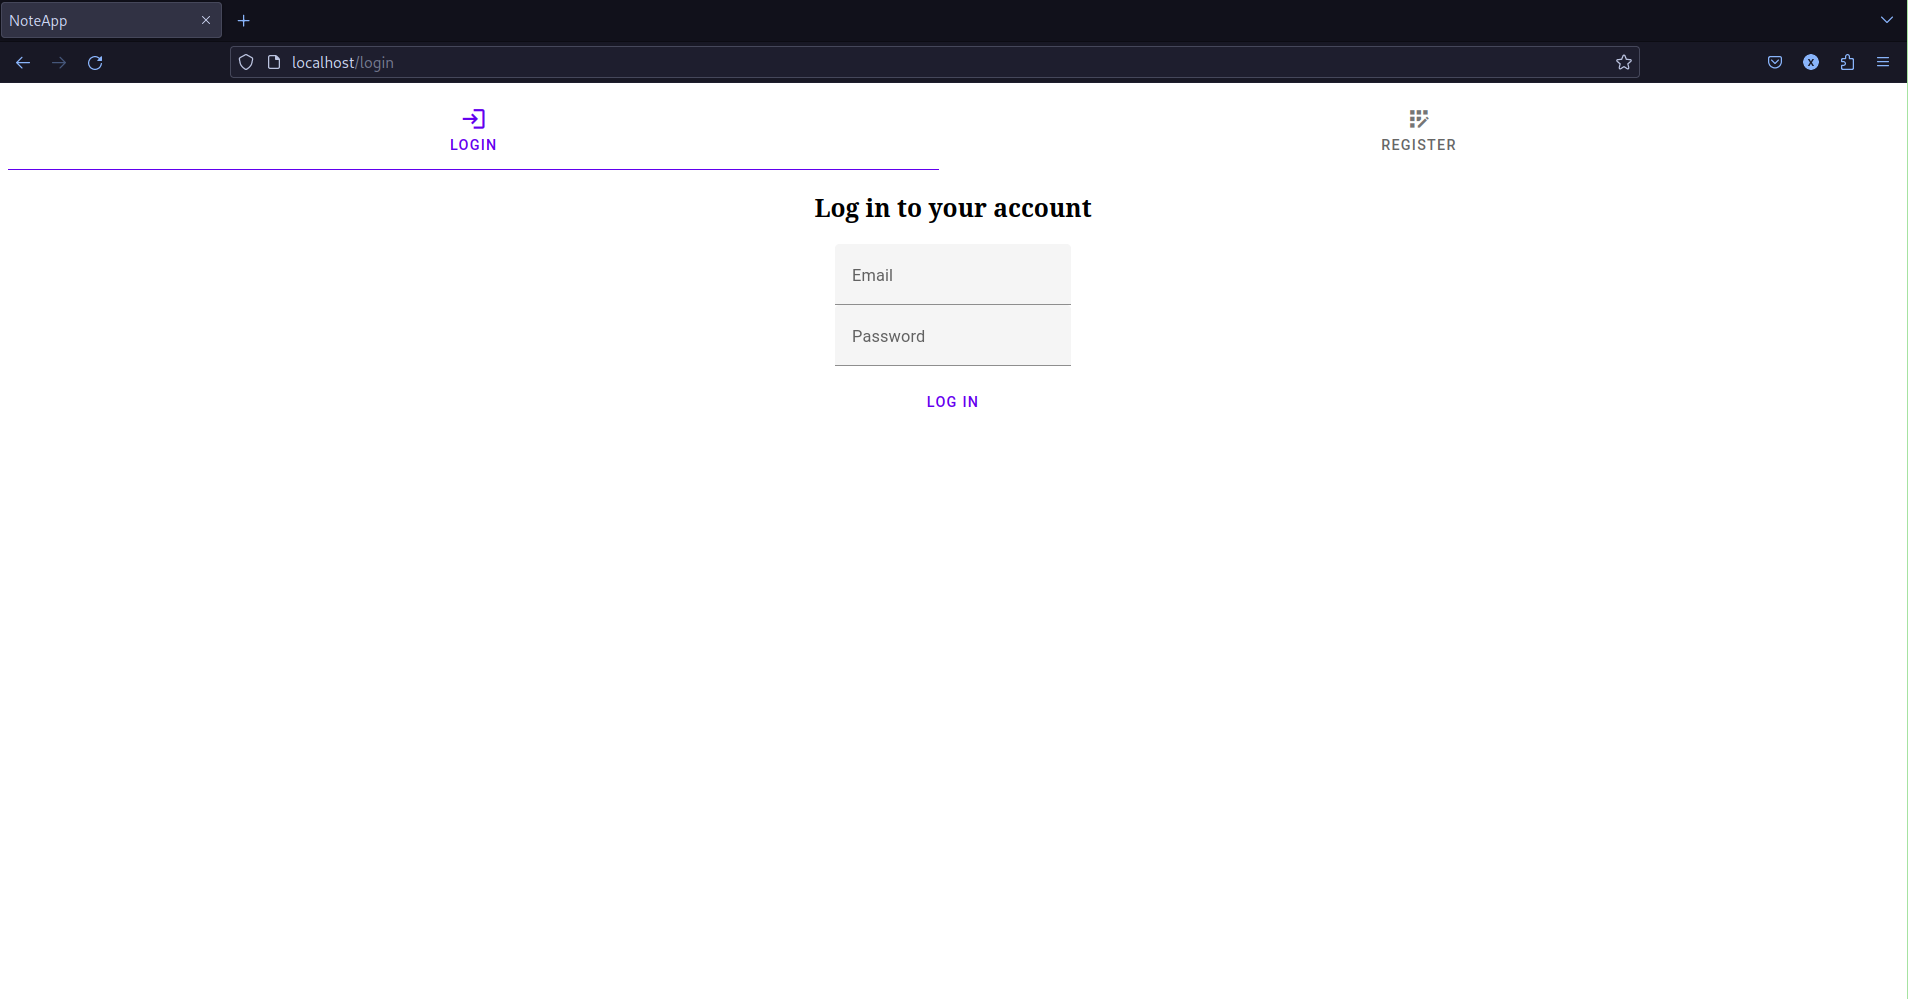
\includegraphics[width=1.0\textwidth]{./images/strona-logowania.png}
\caption{Widok strony logowania}
\label{fig:strona-logowania}
\end{figure}

\begin{figure}[H]
\centering
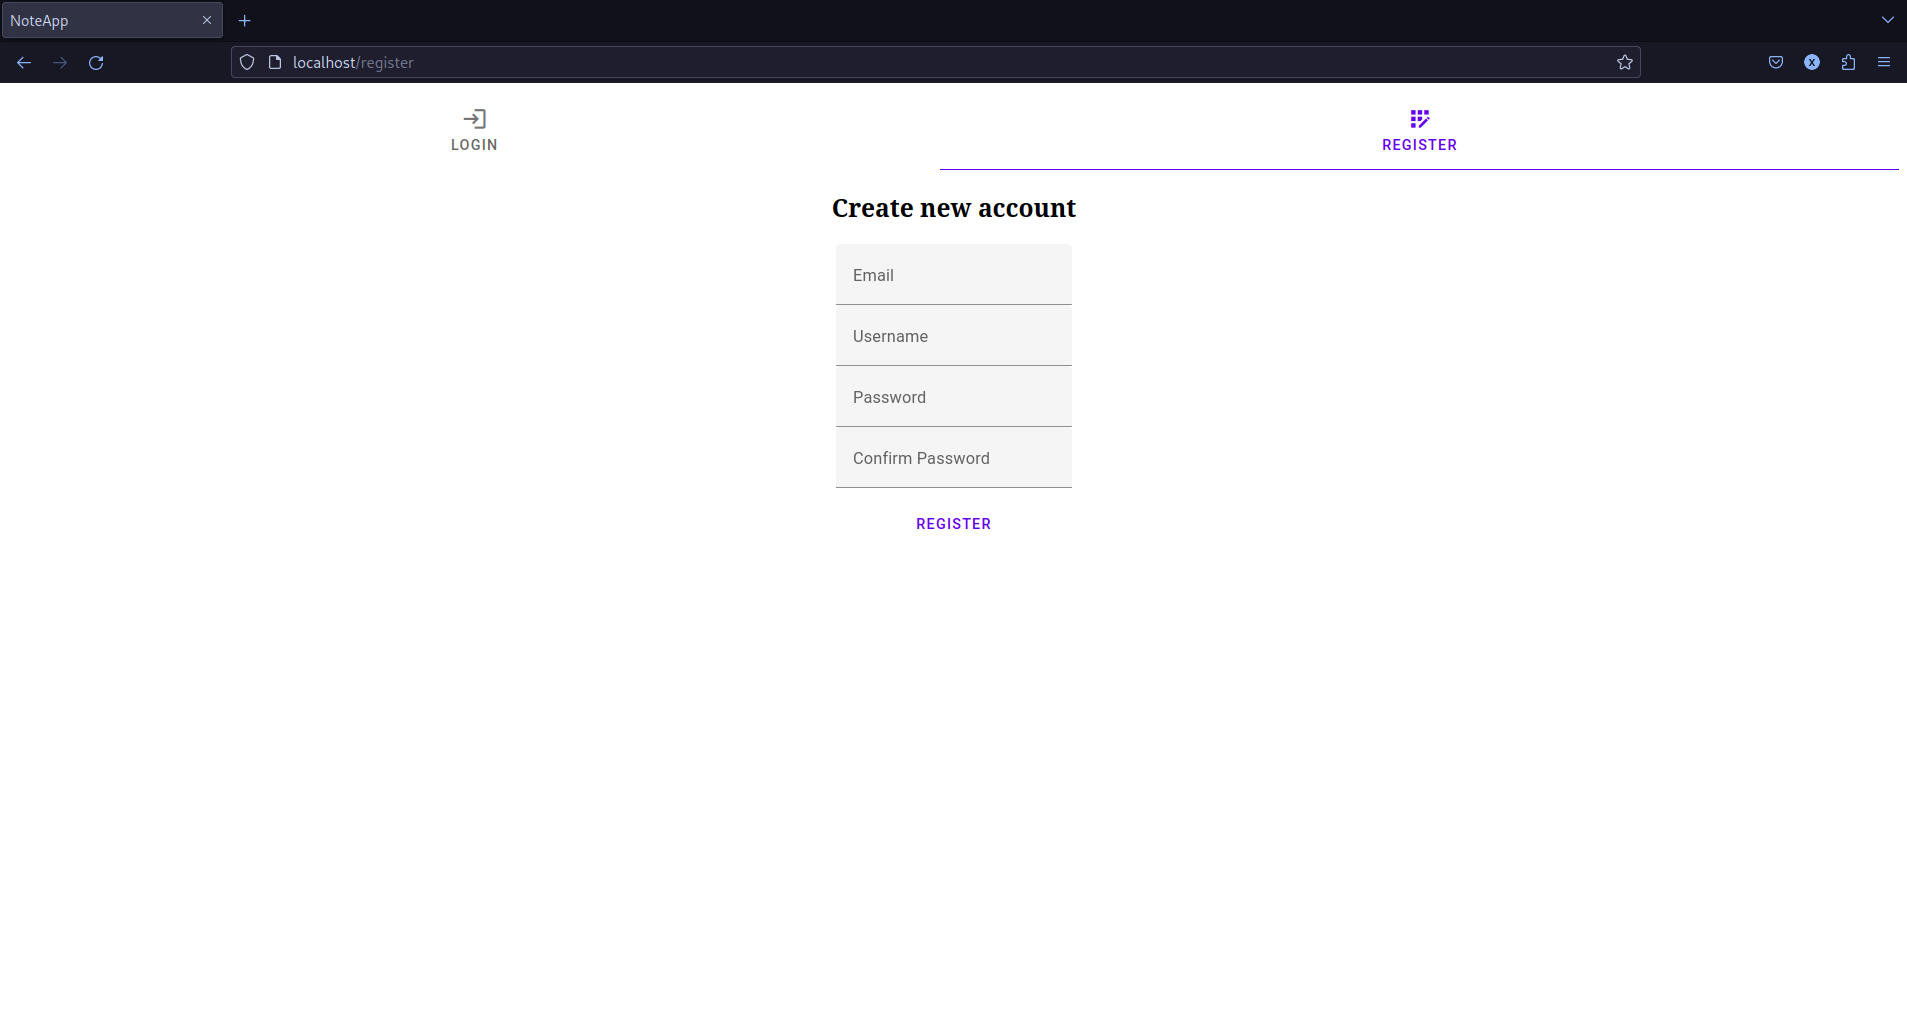
\includegraphics[width=1.0\textwidth]{./images/strona-rejestracji.png}
\caption{Widok strony rejestracji}
\label{fig:strona-rejestracji}
\end{figure}

\subsection{Wyświetlenie, dodawanie i edycja notatek}

Po zalogowaniu użytkownik zobaczy stronę ze swoimi notatkami
(Rys. \ref{fig:strona-notatek}) i (Rys. \ref{fig:strona-dodawania-notatek})

W celu dodania notatki należy wybrać przycisk "+". 
Spowoduje to wyświetlenie strony dodawania notatek (Rys. \ref{fig:strona-dodawania-notatek})

\begin{figure}[H]
\centering
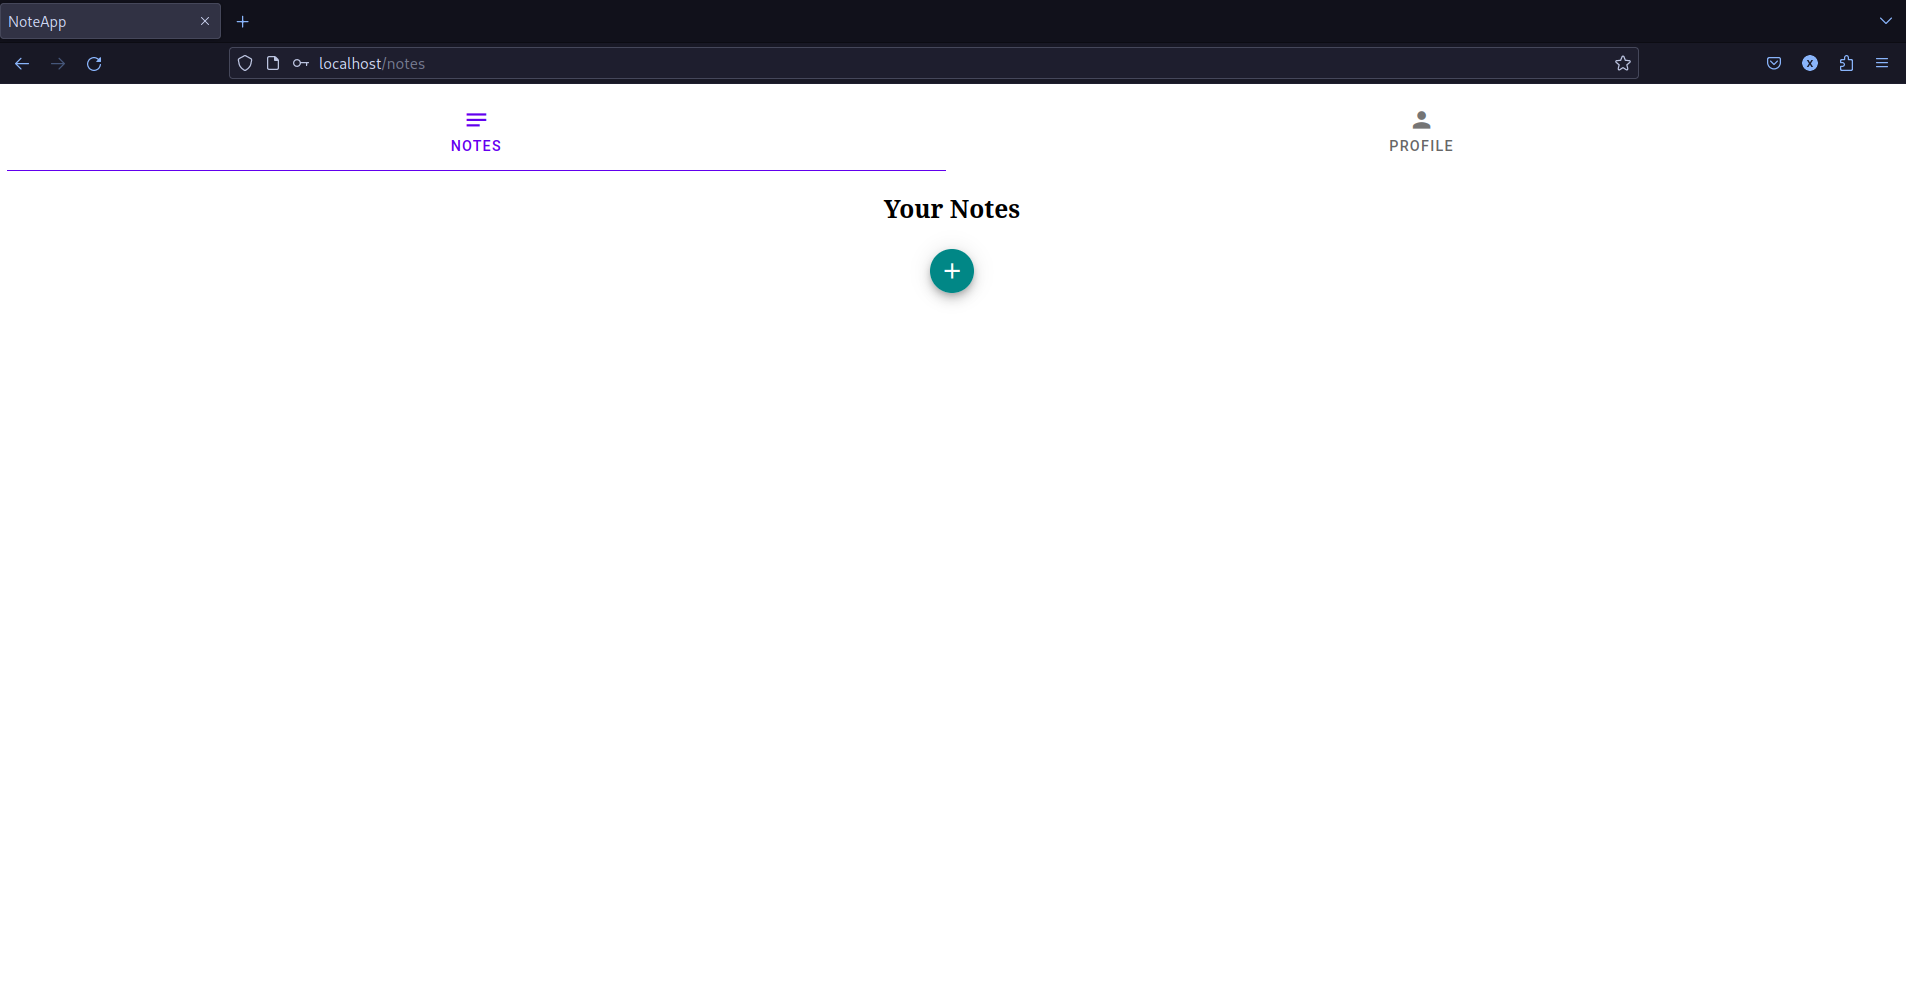
\includegraphics[width=1.0\textwidth]{./images/strona-notatek.png}
\caption{Widok strony notatek (bez notatek)}
\label{fig:strona-notatek}
\end{figure}

\begin{figure}[H]
\centering
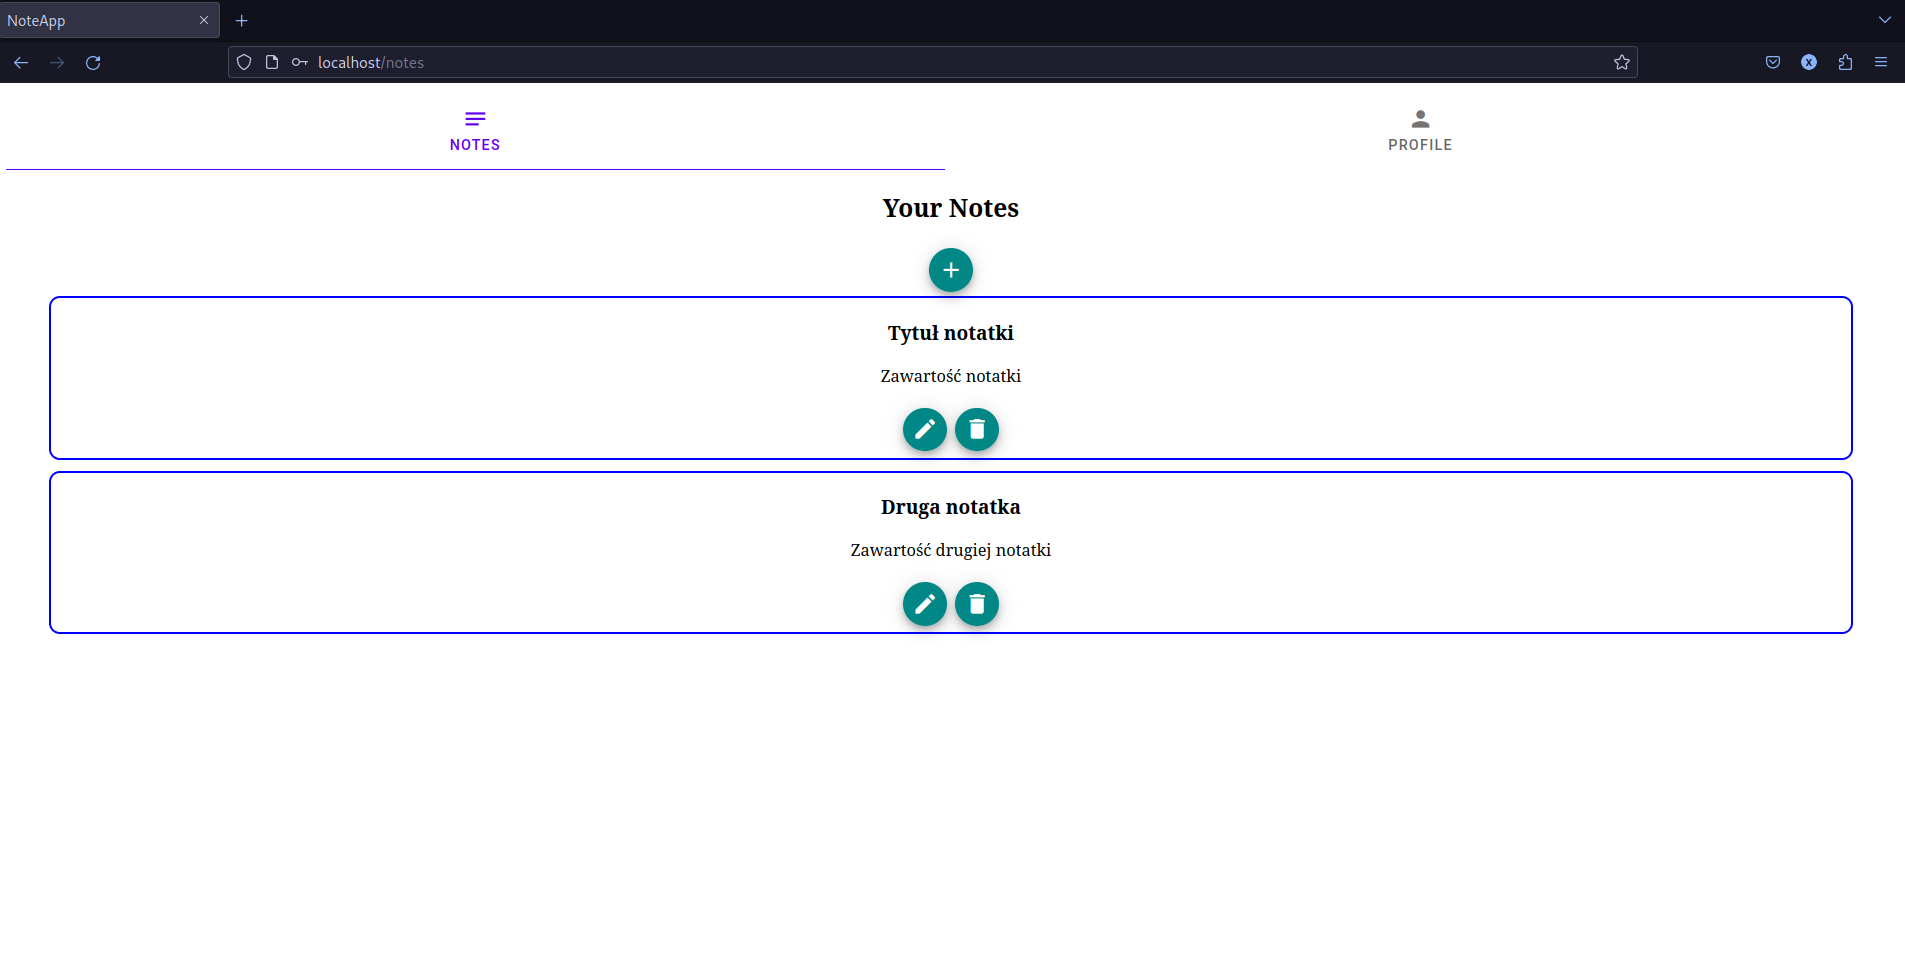
\includegraphics[width=1.0\textwidth]{./images/dodane-notatki.png}
\caption{Widok strony notatek (z dodanymi notatkami)}
\label{fig:strona-notatkek}
\end{figure}

\begin{figure}[H]
\centering
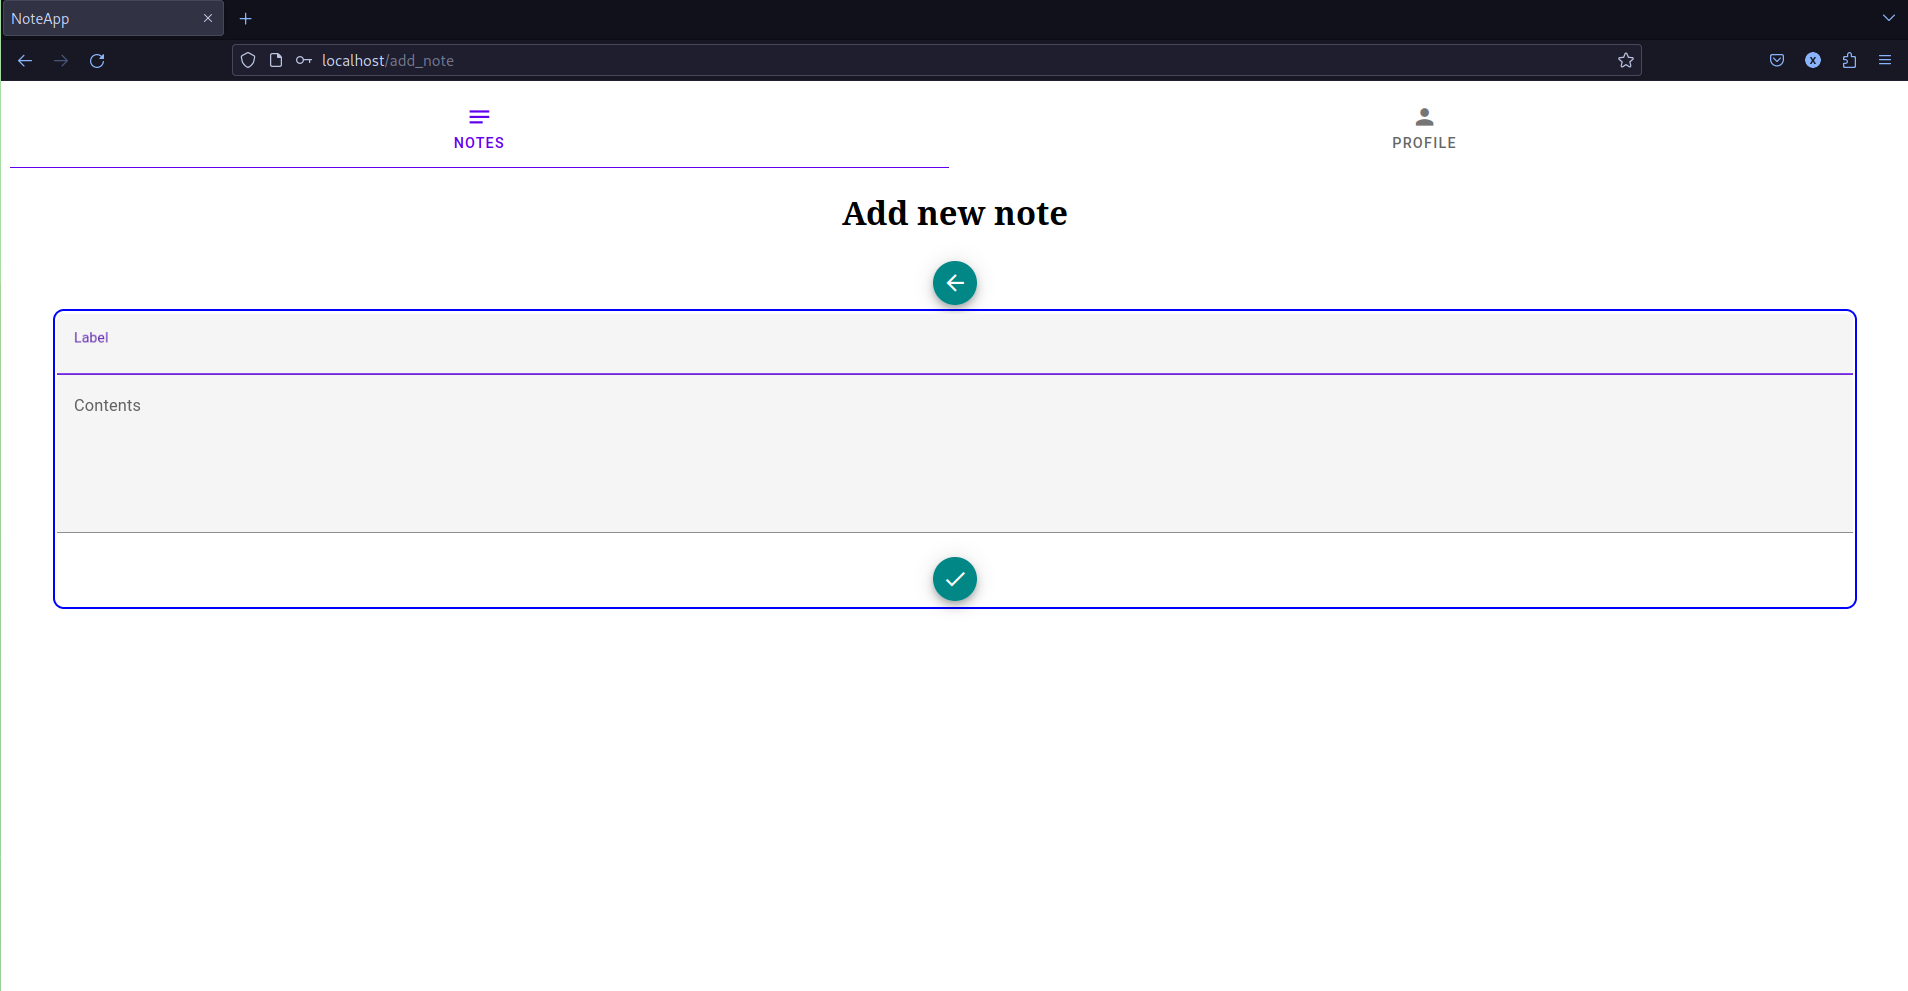
\includegraphics[width=1.0\textwidth]{./images/strona-dodawania-notatek.png}
\caption{Widok strony dodawania notatek}
\label{fig:strona-dodawania-notatek}
\end{figure}

Notatki można edytować i usuwać korzystając z przycisków widocznych na każdej notatce.
Edycja notatki jest przedstawiona na rys. \ref{fig:edycja-notatki}.

\begin{figure}[H]
\centering
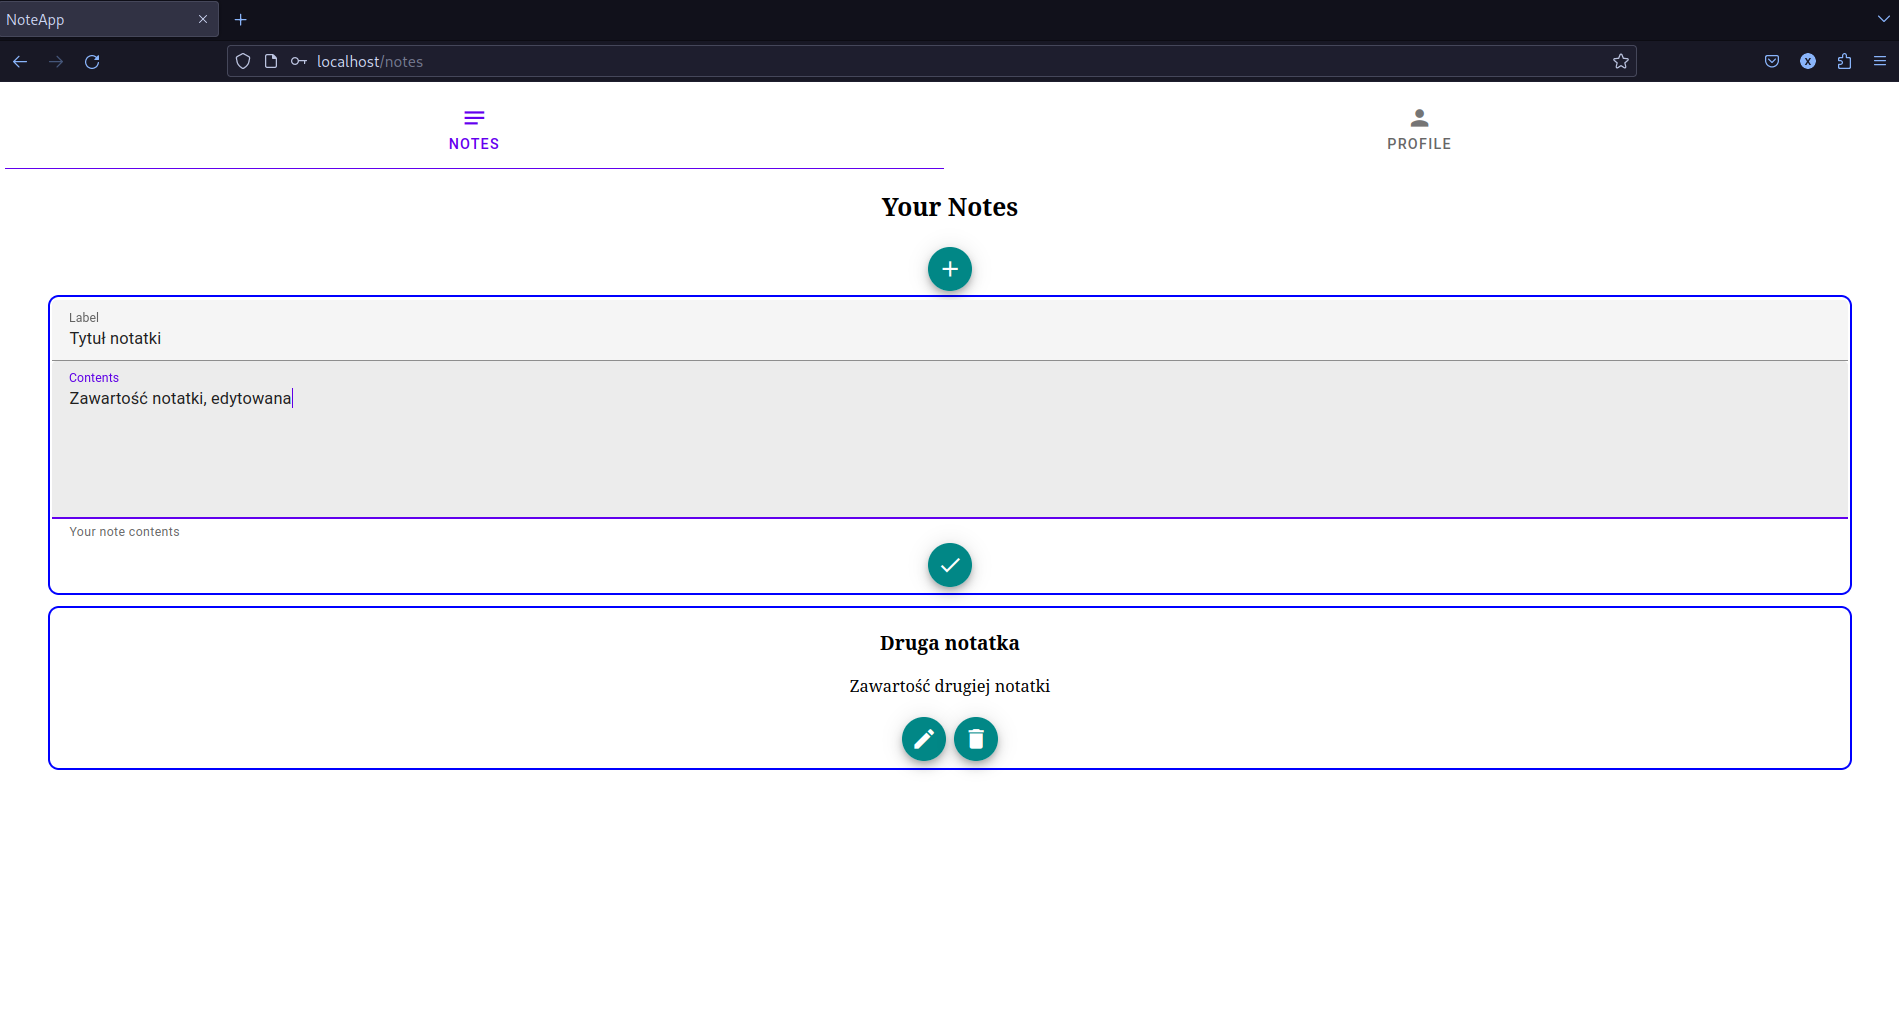
\includegraphics[width=1.0\textwidth]{./images/edycja-notatki.png}
\caption{Edycja notatki}
\label{fig:edycja-notatki}
\end{figure}

\subsection{Zarządzanie profilem}
Widok na profil użytkownika można zobaczyć na Rys. \ref{fig:strona-profilu}. 
Tutaj użytkownik może sprawdzić swoje dane, tutaj również ma możliwość
zarządzania swoim profilem. Możliwe akcje to edycja profilu (Rys \ref{fig:strona-edycja-profilu}),
zmiana hasła, usunięcie profilu lub wylogowanie się z konta.

\begin{figure}[H]
\centering
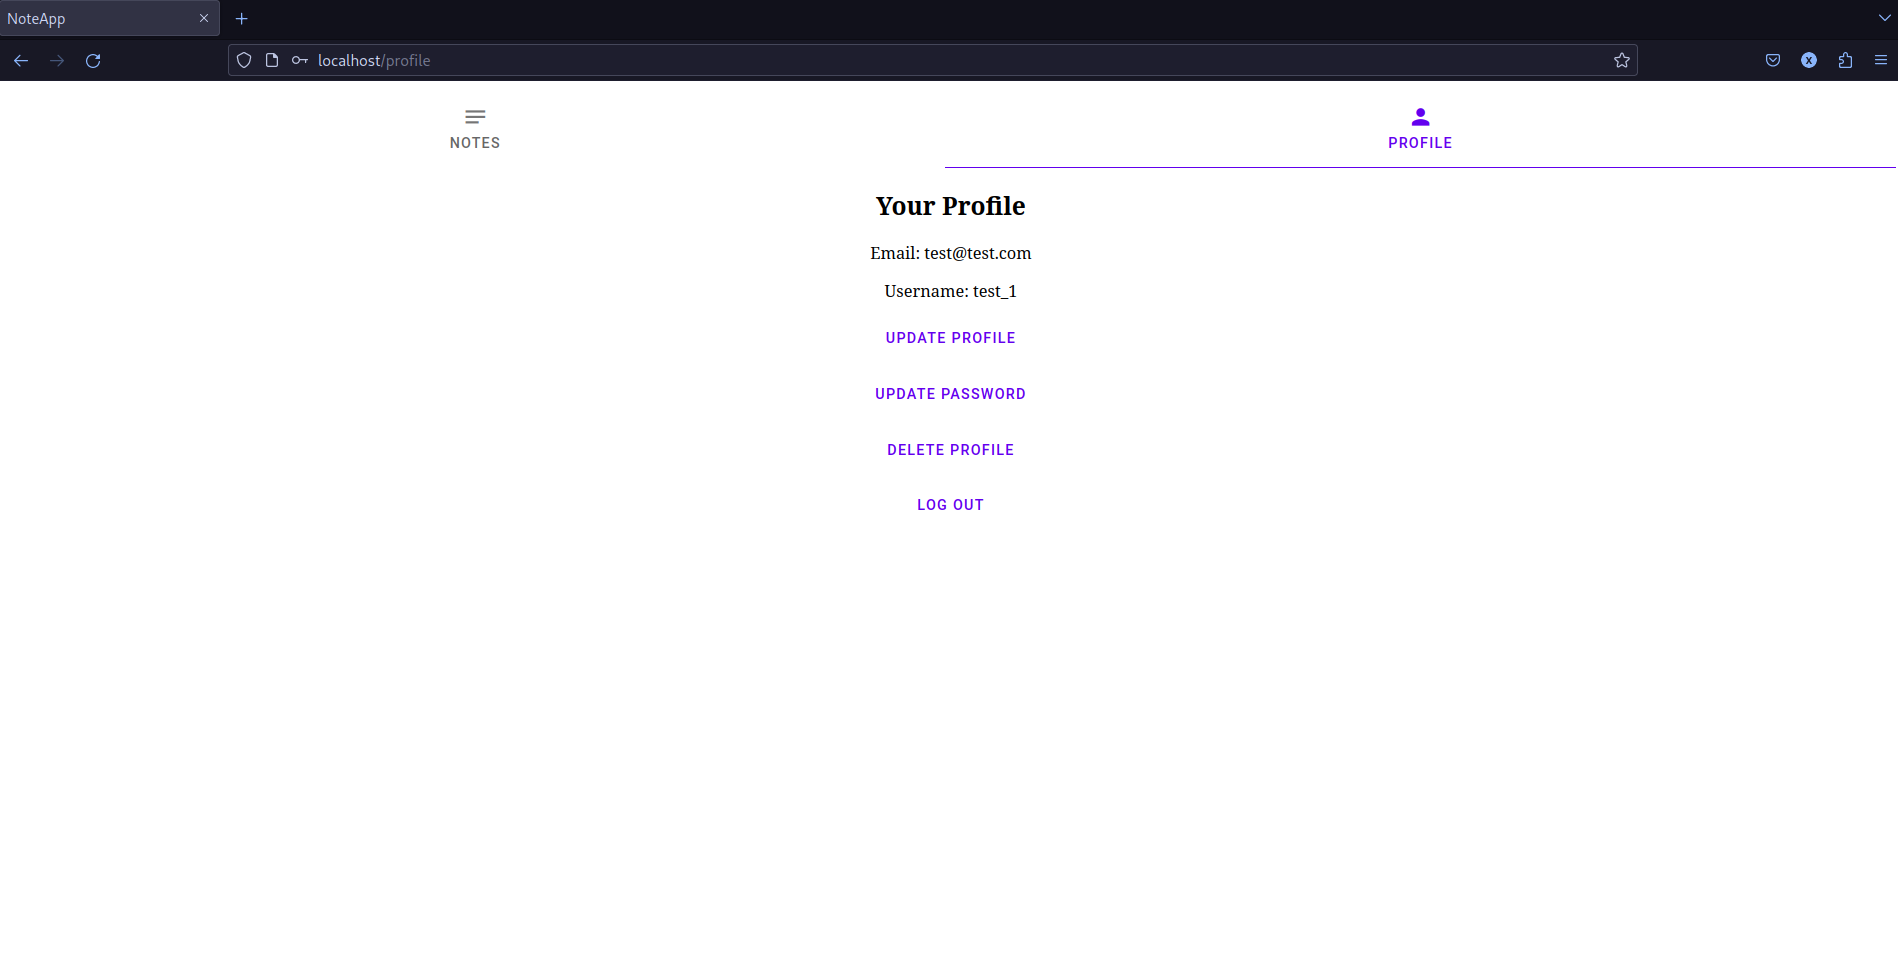
\includegraphics[width=1.0\textwidth]{./images/strona-profilu.png}
\caption{Widok na profil użytkownika}
\label{fig:strona-profilu}
\end{figure}

\begin{figure}[H]
\centering
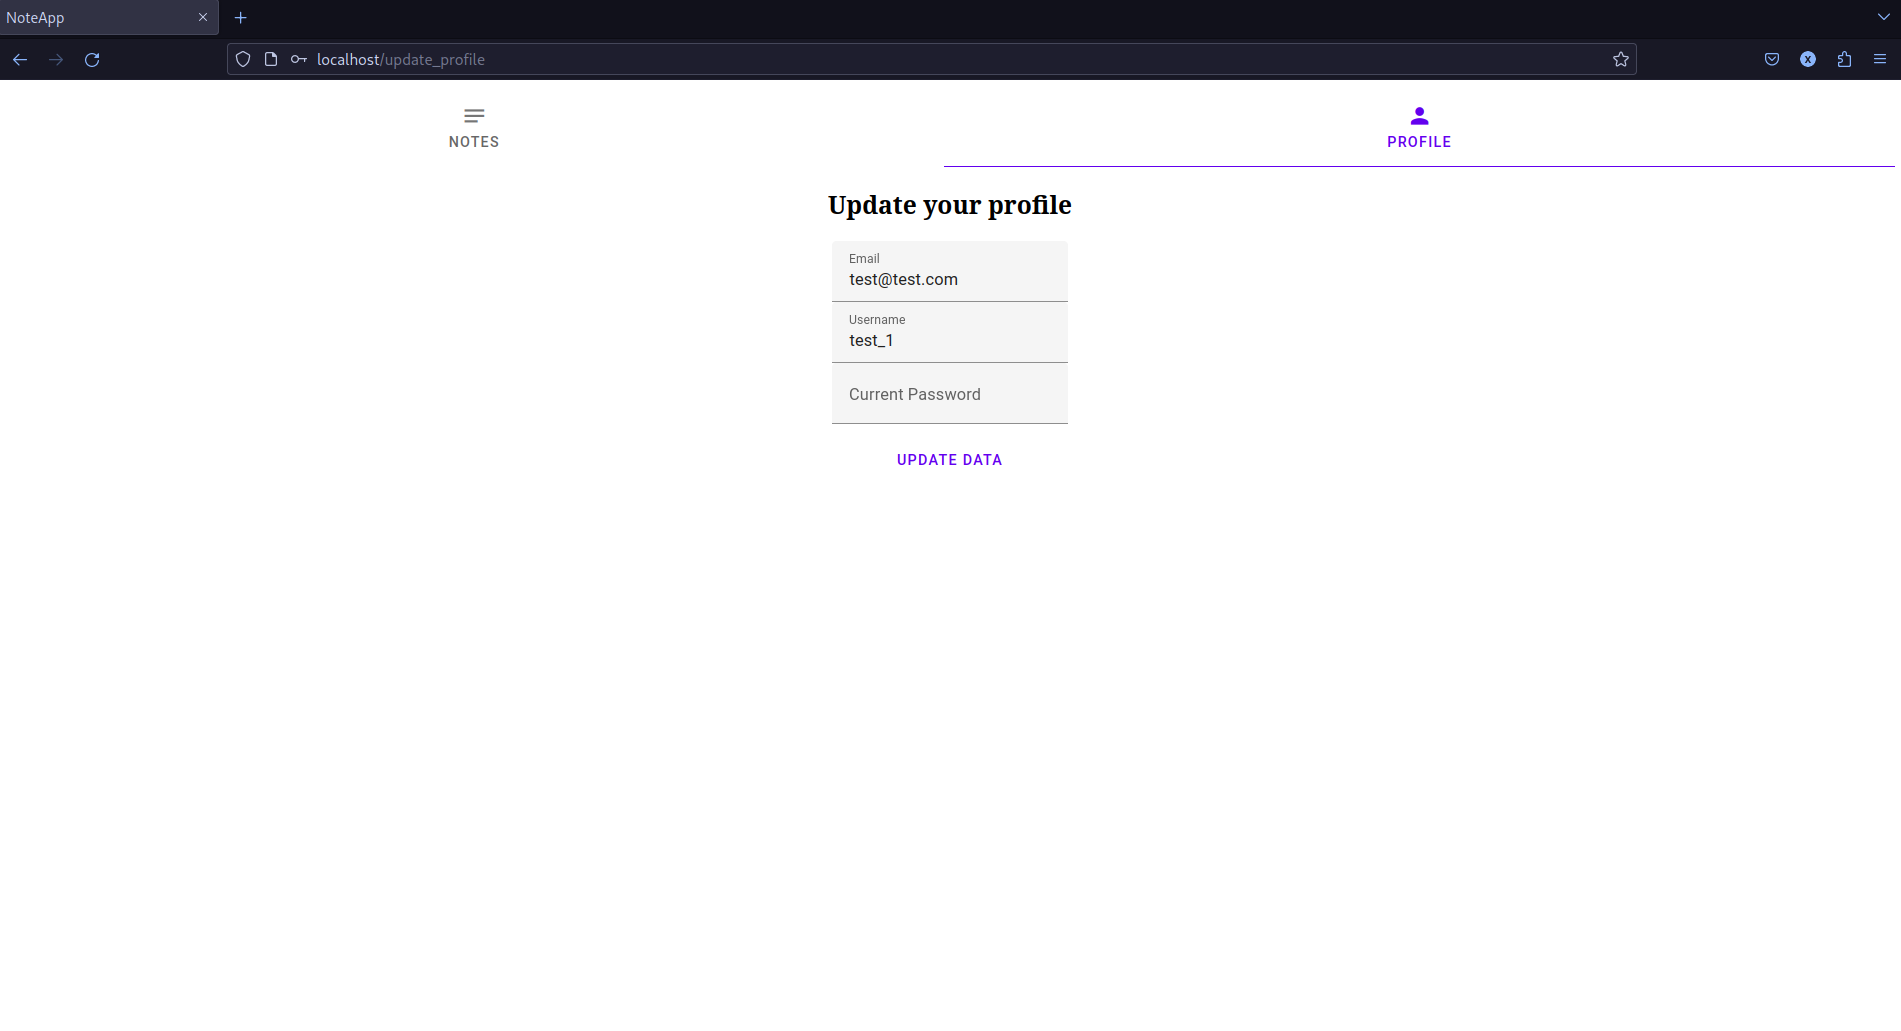
\includegraphics[width=1.0\textwidth]{./images/strona-edycji-profilu.png}
\caption{Widok na stronę edycji profilu użytkownika}
\label{fig:strona-edycja-profilu}
\end{figure}

\section{Administracja systemem}

Systemem można zarządzać za pomocą interfejsu programu Adminer (Rys. \ref{fig:adminer})
Pozwala on na wykonanie dowolnych zapytań SQL na bazie danych programu,
oraz administrację za pomocą czytelnego interfejsu użytkownika.

\begin{figure}[H]
\centering
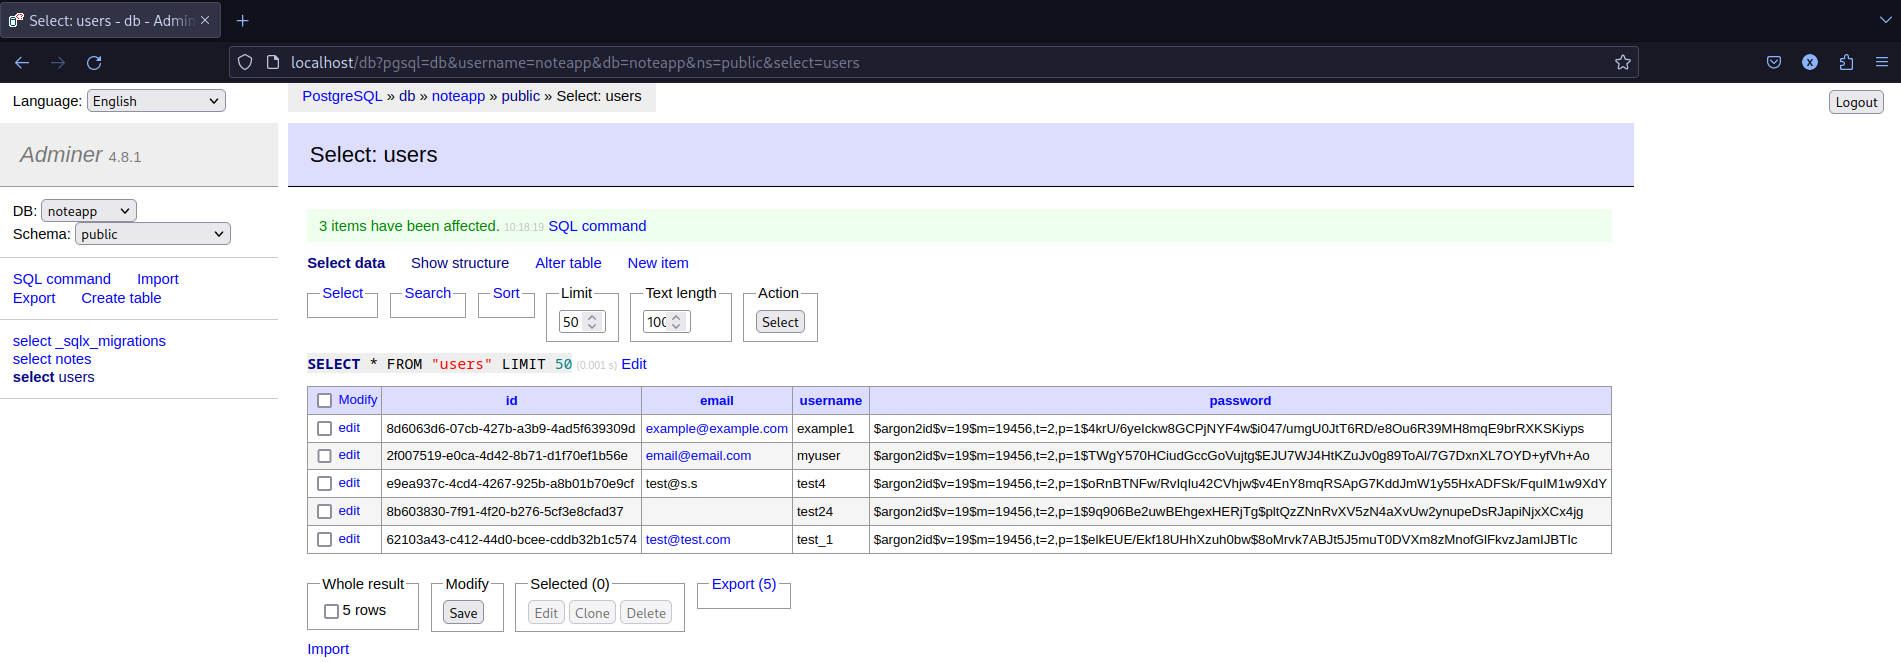
\includegraphics[width=1.0\textwidth]{./images/adminer.png}
\caption{Widok na zarejestrowanych użytkowników - Adminer}
\label{fig:adminer}
\end{figure}

\section{Kwestie bezpieczeństwa}

W aplikacji jest używane wiele zabezpieczeń, których celem jest zapewnienie prywatności
danych przechowywanych w bazie danych, oraz zachowania integralności systemu.

Aplikacja uruchamiana jest korzystajac z platformy Docker, dzięki czemu program jest
odizolowany od reszty systemu. Potencjalny atakujący, jeśli uda mu się w jakikolwiek sposób
uzyskać możliwość wykonywania dowolnego kodu poprzez aplikację, będzie ograniczony do
kontenera, do którego uzyskał dostęp. Nie będzie miał wtedy możliwości spowodowania
szkód na systemie gospodarza.

Drugim elementem chroniącym aplikację jest zastosowanie tokenów JWT do autoryzacji i autentykacji
użytkownika. W celu wykonania jakiejkolwiek operacji jako dany użytkownik, aplikacja pobiera jego
identyfikator z tokenu JWT. Dzięki temu nie jest możliwa jakakolwiek akcja jako dany użytkownik
bez posiadania prawidłowego tokenu. Potencjalną słabością jest użycie nieskomplikowanego hasła 
jako sekretu JWT (JWT\_SECRET). Aby temu zapobiec, zgodnie z zaleceniami z 
sekcji \ref{sec:instalacja} należy ustawić hasło o wysokim poziomie komplikacji dla tej wartości.

Dzięki przechowywaniu haseł użytkownika korzystając z funkcji skrótu Argon 2, w przypadku uzyskania
przez atakującego dostępu do bazy danych hasła są odpowiednio zabezpieczone. 

%%%%%%%%%%%%%%%%%%%%%
%% RYSUNEK Z PLIKU
%
%\begin{figure}
%\centering
%
\includegraphics[width=0.5\textwidth]{./politechnika_sl_logo_bw_pion_pl.pdf}
%\caption{Podpis rysunku zawsze pod rysunkiem.}
%\label{fig:etykieta-rysunku}
%\end{figure}
%Rys. \ref{fig:etykieta-rysunku} przestawia …
%%%%%%%%%%%%%%%%%%%%%
%
%%%%%%%%%%%%%%%%%%%%%
%% WIELE RYSUNKÓW 
%
%\begin{figure}
%\centering
%\begin{subfigure}{0.4\textwidth}
%    
\includegraphics[width=\textwidth]{./politechnika_sl_logo_bw_pion_pl.pdf}
%    \caption{Lewy górny rysunek.}
%    \label{fig:lewy-gorny}
%\end{subfigure}
%\hfill
%\begin{subfigure}{0.4\textwidth}
%    
\includegraphics[width=\textwidth]{./politechnika_sl_logo_bw_pion_pl.pdf}
%    \caption{Prawy górny rysunek.}
%    \label{fig:prawy-gorny}
%\end{subfigure}
%
%\begin{subfigure}{0.4\textwidth}
%    
\includegraphics[width=\textwidth]{./politechnika_sl_logo_bw_pion_pl.pdf}
%    \caption{Lewy dolny rysunek.}
%    \label{fig:lewy-dolny}
%\end{subfigure}
%\hfill
%\begin{subfigure}{0.4\textwidth}
%    
\includegraphics[width=\textwidth]{./politechnika_sl_logo_bw_pion_pl.pdf}
%    \caption{Prawy dolny rysunek.}
%    \label{fig:prawy-dolny}
%\end{subfigure}
%        
%\caption{Wspólny podpis kilku rysunków.}
%\label{fig:wiele-rysunkow}
%\end{figure}
%Rys. \ref{fig:wiele-rysunkow} przestawia wiele ważnych informacji, np. rys. \ref{fig:prawy-gorny} jest na prawo u góry.
%%%%%%%%%%%%%%%%%%%%%


 
%\begin{figure}
%\centering
%\begin{tikzpicture}
%\begin{axis}[
%    y tick label style={
%        /pgf/number format/.cd,
%            fixed,   % po zakomentowaniu os rzednych jest indeksowana wykladniczo
%            fixed zerofill, % 1.0 zamiast 1
%            precision=1,
%        /tikz/.cd
%    },
%    x tick label style={
%        /pgf/number format/.cd,
%            fixed,
%            fixed zerofill,
%            precision=2,
%        /tikz/.cd
%    }
%]
%\addplot [domain=0.0:0.1] {rnd};
%\end{axis} 
%\end{tikzpicture}
%\caption{Podpis rysunku po rysunkiem.}
%\label{fig:2}
%\end{figure}



% TODO
\chapter{Specyfikacja wewnętrzna}
\label{ch:05}

\section{Architektura systemu - Docker}

Architektura jest oparta na platformie Docker.
Każdy z poniższych elementów jest oddzielnym kontenerem:

- nginx - odwrotne proxy, którego rolą jest przekierowywanie zapytań do odpowiednich serwisów, w zależności od ścieżki podanej w URL

- db - zawiera system zarządzający bazą danych PostgreSql

- adminer - system do administracji bazą danych, dzięki któremu można bezpośrednio przegladać i dokonywać zmian w bazie korzystając z graficznego interfejsu użytkownika

- backend - zawiera właściwą aplikację strony serwera (API), oraz wygenerowane pliki strony klienta 

- swagger - system pozwalający na dokumentację i testowanie API

\section{Architektura systemu - implementacja}

Od strony implementacji, projekt jest podzielony na dwie części:

- noteapp-frontend - strona klienta aplikacji

- noteapp-backend - strona serwera aplikacji


\section{Opis bazy danych}

Baza danych składa się z dwóch tabel, reprezentujących użytkowników i notatki.
Każda notatka posiada zapisane id użytkownika, do którego należy (jako klucz obcy).
Diagram bazy danych jest widoczny na Rys. \ref {fig:schemat-bazy}.

\begin{figure}[H]
\centering
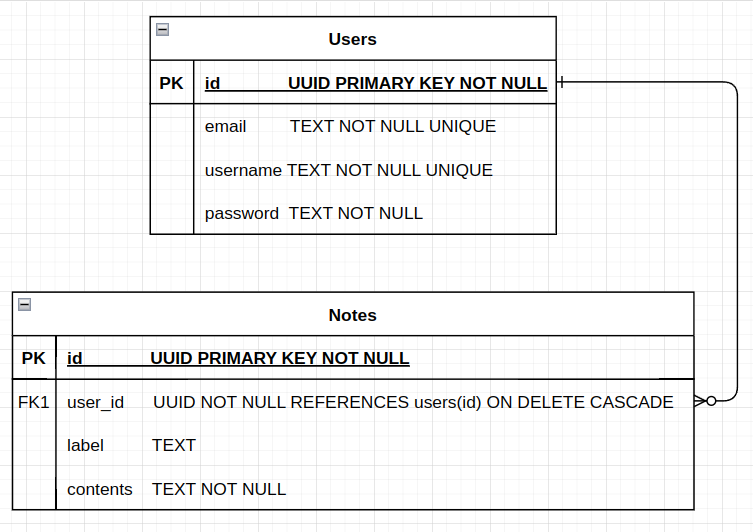
\includegraphics[width=1.0\textwidth]{./images/schemat-bazy.png}
\caption{Schemat bazy danych}
\label{fig:schemat-bazy}
\end{figure}


\section{Najważniejsze biblioteki i moduły}
\subsection{Yew}

Yew to framework pozwalający na tworzenie strony klienta aplikacji internetowej.
Poniżej wypisano jego najważniejsze cechy:

- jest frameworkiem napisanym w języku Rust, co oznacza,
że programista otrzymuje korzyści z bezpieczeństwa i wydajności tego języka.

- wspiera programowanie reaktywne, co oznacza, że można łatwo obsługiwać zmiany stanu i automatycznie aktualizować interfejs użytkownika w zależności od tych zmian.

- opiera się na koncepcji komponentów, co ułatwia strukturyzację kodu i jego ponowne użycie. Komponenty mogą zawierać zarówno logikę, jak i szablony HTML.

- używa wirtualnego drzewa DOM (Virtual DOM), co pozwala na efektywne aktualizacje interfejsu użytkownika poprzez porównywanie zmian w drzewie DOM przed i po aktualizacji.

- pozwala na asynchroniczną komunikację z serwerem

Strona frameworku: \url{https://yew.rs/}.

\subsection{Axum}

Axum to framework pozwalający na tworzenie strony serwera aplikacji internetowej.
Jego głównymi założeniami są ergonomia i modularność. Pozwala w łatwy sposób 
tworzyć API aplikacji, oraz kotrolować interakcję z użytkownikiem zarówno na niskim,
jak i wysokim poziomie abstrakcji. Framework wymaga użycia asynchroniczności podczas
tworzenia aplikacji, dzięki czemu może być obsługiwanych wiele zapytań jednocześnie.

Strona repozytorium frameworku: \url{https://github.com/tokio-rs/axum}.

\section{Najważniejsze klasy}

Najważniejsze klasy zaimplementowane w aplikacji spełniają funkcję interfejsowania
z bazą danych (Rys. \ref{fig:pseudokod:klasa-note}, Rys. \ref{fig:pseudokod:klasa-user}) lub z zapytaniami użytkownika (Rys. \ref{fig:pseudokod:klasa-interact-user}, Rys. \ref{fig:pseudokod:klasa-interact-note}).


\section{Szczegóły implementacji - logowanie}

Logowanie jest kluczowym elementem wielu aplikacji intenetowych,
gdyż od bezpieczeństwa jego implementacji zależy prywatność i nienaruszalność
informacji powierzonych aplikacji przez użytkownika.

Fragment kodu odpowiedzialny za obsługę zapytań logowania:

\begin{figure}[H]
\centering
\begin{lstlisting}
pub (super) async fn login(
    Extension(pool): Extension<PgPool>,
    Json(LoginRequest{email, password}): Json<LoginRequest>
) -> Result<impl IntoResponse, ApiError> {
    let credentials = User::select_credentials(&email, &pool).await
        .map_err(|_| ApiError::InvalidCredentials)?;
    
    if authenticate(&password, &credentials.password).await? {
        let token = generate_token(credentials.id);
        let cookie = generate_auth_cookie(&token);

        let mut response = Response::new(json!({"status": "success", "token": token}).to_string());

        response
            .headers_mut()
            .insert(header::SET_COOKIE, cookie.to_string().parse().unwrap());

        return Ok(response);
    }

    return Err(ApiError::InvalidCredentials)
}
\end{lstlisting}
\caption{Obsługa zapytań logowania}
\label{fig:pseudokod:logowanie}
\end{figure}

Na początku z bazy danych pobierane są dane logowania użytkownika na podstawie podanego
adresu email. Następnie, funkcji authenticate() jest przekazywane hasło (wynik funkcji skrótu)
pobrane z bazy danych, oraz hasło podane przez użytkownika podczas próby logowania. 
Jeżeli wynik funkcji skrótu Argon 2 dla hasła podanego przez użytkownika jest taki sam
jak wynik pobrany z bazy danych, funkcja authenticate() zwróci wartość "true", w przeciwnym
wypadku "false". 

Następnym etapem, jeśli autentykacja się powiodła, jest skonstruowanie i zwrócenie
użytkownikowi tokenu JWT uprawniającego go do korzystania z funkcjonalności aplikacji
jako zalogowany użytkownik. W przypadku błędu spowodowanego nieprawidłowymi danymi
na którymkolwiek etapie logowania, aplikacja zwróci błąd informujący o podaniu niewłaściwych
danych logowania. Wiadomość ta nie będzie się różnić, niezależnie od tego czy nieprawidłowy
jest użyty adres email czy też hasło, aby zapobiec możliwości enumeracji prawidłowych
(obecnych w bazie danych) adresów email przez potencjalnego atakującego.

% % % % % % % % % % % % % % % % % % % % % % % % % % % % % % % % % % % 
% Pakiet minted wymaga importu: \usepackage{minted}                 %
% i specjalnego kompilowania:                                       %
% pdflatex -shell-escape main                                       %
% % % % % % % % % % % % % % % % % % % % % % % % % % % % % % % % % % % 

%\begin{figure}
%\centering
%\begin{minted}[linenos,frame=lines]{c++}
%class test : public basic
%{
%    public:
%      test (int a);
%      friend std::ostream operator<<(std::ostream & s, 
%                                     const test & t);
%    protected:
%      int _a;  
%      
%};
%\end{minted}
%\caption{Pseudokod w \texttt{minted}.}
%\label{fig:pseudokod:minted}
%\end{figure}




\chapter{Weryfikacja i walidacja}
\label{ch:06}

\section{Sposób testowania}
\subsection{Testowanie strony serwera}
Program był testowany na wiele sposobów. Na początku tworzona była strona serwera,
którą testowano za pomocą narzędzi swagger oraz curl. 

Głównym kryterium podczas testowania była poprawność reakcji serwera w odpowiedzi
na różnego rodzaju, właściwie i niewłaściwie przygotowane dane. 

Sprawdzana również była zawartość bazy danych pod względem ciągłości przekazywanych
przez użytkownika danych. Weryfikowana było również, czy hasła są odpowiednio preparowane
przed zapisaniem w bazie danych (użycie przez program funkcji skrótu Argon2), zarówno
podczas rejestracji jak i zabiegu zmiany hasła. Program był również testowany pod względem
różnych ataków, na przykład możliwości obejścia logowania, czy też dostępu do danych użytkownika
obecnego w systemie bez posiadania jego danych logowania.

Przetestowano każdą dostępną dla użytkownika funkcjonalność 
i stwierdzono poprawność jej działania.

\subsection{Testowanie strony klienta}

Testowanie strony klienta odbywało się poprzez użycie narzędzi developerskich dostępnych
w przeglądarce Firefox, oraz za pomocą serwera do testowania i rozwijania aplikacji
zapewnianego przez narzędzie Trunk. Każdy punkt kontaktu z serwerem został przetestowany
pod względem poprawnego działania zgodnie z logiką aplikacji. Przetestowano zachowanie
aplikacji podczas odświeżania, a także nawigacji na poprzednią/następną stronę.
Szczególną uwagę poświęcono zadbaniu, aby strona klienta aplikacji nie wylogowywała 
użytkownika po odświeżeniu strony.

\section{Wykryte i usunięte błędy}
\subsection{Niepoprawnie działające logowanie}
Początkowa implementacja logowania użytkownika nie pozwalała na poprawną
autentykację nawet przy podaniu poprawnych danych logowania. Zamiast tego
pozwalała na zalogowanie po podaniu poprawnego adresu email wraz ze wynikiem
funkcji skrótu Argon 2 zamiast hasła. Błąd ten był spowodowany niewłaściwym 
zrozumieniem działania funkcji weryfikacji poprawności hasła dostarczanej
przez użytą bibliotekę implementującą Argon 2 dla języka Rust, co doprowadziło
do decyzji o haszowaniu podanego przez użytkownika hasła, a potem 
zweryfikowaniu go z haszem pobranym z bazy danych.

Problem ten rozwiązano usuwając fragment kodu haszujący podane przez użytkownika
hasło, gdyż po dokładnym przeczytaniu dokumentacji zrozumiano, że należy jako
argumenty do niej podać hash pobrany z bazy danych wraz z hasłem podanym przez
użytkownika bez żadnych dodakowych modyfikacji.

\subsection{Wylogowanie użytkownika po odświeżeniu strony}
Aplikacja, po odświeżeniu strony przenosiła użytkownika na stronę logowania,
nie pozwalając mu na przeglądanie notatek, profilu ani dokonywanie jakichkolwiek
zmian, mimo posiadania odpowiedniego tokenu potwierdzającego jego toższamość.
Zachowanie te było spowodowane sposobem przechowywania informacji o stanie zalogowana
użytkownika po stronie klienta aplikacji. Informacja ta była automatycznie usuwana
przy restarcie (odświeżeniu) strony klienta.

Problem ten rozwiązano poprzez wykonanie zapytania o informacje użytkownika
do serwera na samym początku cyklu życia klienta. Jeżeli przeglądarka miała
zapisany aktualny token, serwer odpowiadał danymi użytkownika tego tokenu, 
w przeciwnym wypadku serwer odpowiadał kodem błędu. Po wykonaniu tego
zapytania, zależnie od odpowiedzi, strona klienta ustawia początkową
wartość stanu zalogowania użytkownika, po czym wykonywane są odpowiednie
akcje (wyświetlenie strony z notatkami użytkownika, lub wyświetlenie strony
logowania).


\chapter{Podsumowanie i wnioski}
\section{Weryfikacja wymagań}
\subsection{Wymagania funkcjonalne}

Wszystkie wymagania funkcjonalne aplikacji zostały spełnione:

- aplikacja pozwala użytkownikowi na tworzenie, modyfikację, przeglądanie i usuwanie notatek

- aby skorzystać z aplikacji, wymagana jest rejestracja oraz logowanie

- użytkownik może przeglądać, modyfikować oraz usunąć swój profil

- zaimplementowane są mechanizmy zabezpieczające prywatność danych użytkownika i jego notatek

- nie jest możliwe wprowadzenie zmian w profilu użytkownika oraz zmiany hasła bez podania
obecnego hasła użytkownika

\subsection{Wymagania niefunkcjonalne}

Wszystkie wymagania niefunkcjonalne aplikacji zostały spełnione:

- jest możliwość uruchomienia programu na dowolnym systemie, o ile obsługuje on platformę Docker w odpowiedniej wersji

- interakcja użytkowników ze stroną serwera aplikacji oraz serwera aplikacji z serwerem bazy 
danych odbywa się asynchronicznie, dzięki użyciu asynchronicznych funkcjonalności języka Rust i frameworku Axum

- strona serwera aplikacji jest odizolowana od reszty systemu dzięki użyciu funkcjonalności
kontenryzacji platformy Docker


\section{Kierunki rozwoju}

- implementacja funkcjonalności udostępniania notatek innym użytkownikom

- dodanie proszego w obsłudze i bliżej zintegrowanego z aplikacją systemu administracji

- poprawa wyglądu i dodanie możliwości personalizacji interfejsu użytkownika aplikacji


\backmatter

%\bibliographystyle{plplain}  % bibtex
%\bibliography{biblio} % bibtex
% \printbibliography           % biblatex
% \addcontentsline{toc}{chapter}{Bibliografia}

\begin{appendices}

\chapter{Spis skrótów i symboli}

% \begin{itemize}
% \end{itemize}


\chapter{Źródła}

\begin{figure}[H]
\centering
\begin{lstlisting}
#[derive(FromRow, Serialize, Deserialize, Debug)]
pub struct Note {
    pub id: Uuid,
    pub label: Option<String>,
    pub contents: String,
    pub user_id: Uuid
}
\end{lstlisting}
\caption{Klasy do interakcji z tabelą notatek}
\label{fig:pseudokod:klasa-note}
\end{figure}

\begin{figure}[H]
\centering
\begin{lstlisting}
#[derive(FromRow, Debug, Serialize)]
pub struct UserProfile {
    pub id: Uuid,
    pub email: String,
    pub username: String
}

#[derive(FromRow, Serialize, Deserialize, Debug)]
pub struct Credentials {
    pub id: Uuid,
    pub email: String,
    pub password: String,
}
\end{lstlisting}
\caption{Klasy do interakcji z tabelą użytkownika}
\label{fig:pseudokod:klasa-user}
\end{figure}

\begin{figure}[H]
\centering
\begin{lstlisting}
#[derive(Deserialize, Debug)]
pub(super) struct UserRequest {
    pub email: String,
    pub username: String,
    pub password: String,
}

#[derive(Deserialize, Debug)]
pub(super) struct LoginRequest {
    pub email: String,
    pub password: String,
}

#[derive(Deserialize, Debug)]
pub(super) struct UpdatePasswordRequest {
    pub password: String,
    pub new_password: String,
}

#[derive(Deserialize, Debug)]
pub(super) struct AnyPassword {
    pub password: String,
}
\end{lstlisting}
\caption{Klasy do interakcji z zapytaniami dotyczącymi użytkownika}
\label{fig:pseudokod:klasa-interact-user}
\end{figure}

\begin{figure}[H]
\centering
\begin{lstlisting}
#[derive(Serialize, Deserialize, Debug)]
pub(super) struct NewNote {
    pub label: Option<String>,
    pub contents: String,
}

#[derive(Serialize, Deserialize, Debug)]
pub(super) struct UpdateNote {
    pub id: Uuid,
    pub label: Option<String>,
    pub contents: String,
}
\end{lstlisting}
\caption{Klasy do interakcji z zapytaniami dotyczącymi notatek}
\label{fig:pseudokod:klasa-interact-note}
\end{figure}

% % % % % % % % % % % % % % % % % % % % % % % % % % % % % % % % % % % 
% Pakiet minted wymaga odkomentowania w pliku config/settings.tex   %
% importu pakietu minted: \usepackage{minted}                       %
% i specjalnego kompilowania:                                       %
% pdflatex -shell-escape praca                                      %
% % % % % % % % % % % % % % % % % % % % % % % % % % % % % % % % % % % 

%\begin{minted}[linenos,breaklines,frame=lines]{c++}
%if (_nClusters < 1)
%   throw std::string ("unknown number of clusters");
%if (_nIterations < 1 and _epsilon < 0)
%   throw std::string ("You should set a maximal number of iteration or minimal difference -- epsilon.");
%if (_nIterations > 0 and _epsilon > 0)
%   throw std::string ("Both number of iterations and minimal epsilon set -- you should set either number of iterations or minimal epsilon.");
%\end{minted}


% TODO
\chapter{Lista dodatkowych plików, uzupełniających tekst pracy} 

Do pracy dołączono następujące pliki:

- kod źródłowy strony klienta

- kod źródłowy strony serwera

- krótkie nagranie prezentujące korzystanie z aplikacji

- pliki konfiguracyjne dla platformy Docker i innych narzędzi

\listoffigures
\addcontentsline{toc}{chapter}{Spis rysunków}
\listoftables
\addcontentsline{toc}{chapter}{Spis tabel}

\end{appendices}

\end{document}


%% Finis coronat opus.

